\documentclass[10pt, landscape]{article}
\usepackage[scaled=0.92]{helvet}
\usepackage{calc}
\usepackage{multicol}
\usepackage{ifthen}
\usepackage[a4paper,margin=5mm,landscape]{geometry}
\usepackage{amsmath,amsthm,amsfonts,amssymb}
\usepackage{color,graphicx,overpic}
\usepackage{hyperref}
\usepackage{newtxtext} 
\usepackage{enumitem}
\usepackage{amssymb}
\usepackage[table]{xcolor}
\usepackage{vwcol}
\usepackage{tikz}
\usetikzlibrary{arrows.meta}
\usetikzlibrary{calc}
\usepackage{mathtools}
\usepackage{nicematrix}
\usepackage[T1]{fontenc} %%% <--- NOTE THIS
% for relations
\usepackage{cancel}
\usepackage{ mathrsfs }
\usepackage{listings}
\usepackage{background}
\setlist{nosep}

\usepackage{etoolbox}
\makeatletter
\preto{\@verbatim}{\topsep=0pt \partopsep=0pt }
\makeatother

\backgroundsetup{
scale=1,
color=black,
opacity=0.4,
angle=0,
contents={}
}

\pdfinfo{
  /Title (MA3205.pdf)
  /Creator (TeX)
  /Producer (pdfTeX 1.40.0)
  /Author (Seamus)
  /Subject (Example)
  /Keywords (pdflatex, latex,pdftex,tex)}

\lstset{language=Java,keywordstyle={\bfseries \color{black}}}

% Turn off header and footer
\pagestyle{empty}

\newenvironment{tightcenter}{%
  \setlength\topsep{0pt}
  \setlength\parskip{0pt}
  \begin{center}
}{%
  \end{center}
}

% redefine section commands to use less space
\makeatletter
\renewcommand{\section}{\@startsection{section}{1}{0mm}%
                                {-1ex plus -.5ex minus -.2ex}%
                                {0.5ex plus .2ex}%x
                                {\normalfont\large\bfseries}}
\renewcommand{\section}{\@startsection{section}{2}{0mm}%
                                {-1explus -.5ex minus -.2ex}%
                                {0.5ex plus .2ex}%
                                {\normalfont\normalsize\bfseries}}
\renewcommand{\subsection}{\@startsection{subsection}{3}{0mm}%
                                {-1ex plus -.5ex minus -.2ex}%
                                {1ex plus .2ex}%
                                {\normalfont\small\bfseries}}%
\renewcommand{\familydefault}{\sfdefault}
\renewcommand\rmdefault{\sfdefault}
% makes nested numbering (e.g. 1.1.1, 1.1.2, etc)
\renewcommand{\labelenumii}{\theenumii}
\renewcommand{\theenumii}{\theenumi.\arabic{enumii}.}
\renewcommand\labelitemii{•}
%  for logical not operator
\renewcommand{\lnot}{\mathord{\sim}}
\renewcommand{\bf}[1]{\textbf{#1}}
\newcommand{\abs}[1]{\vert #1 \vert}
\newcommand{\Mod}[1]{\ \mathrm{mod}\ #1}

\makeatother
\definecolor{myblue}{cmyk}{1,.72,0,.38}
\everymath\expandafter{\the\everymath \color{myblue}}
% Define BibTeX command
\def\BibTeX{{\rm B\kern-.05em{\sc i\kern-.025em b}\kern-.08em
    T\kern-.1667em\lower.7ex\hbox{E}\kern-.125emX}}
\let\iff\leftrightarrow
\let\Iff\Leftrightarrow
\let\then\rightarrow
\let\Then\Rightarrow

% Don't print section numbers
\setcounter{secnumdepth}{0}

\setlength{\parindent}{0pt}
\setlength{\parskip}{0pt plus 0.5ex}
%% this changes all items (enumerate and itemize)
\setlength{\leftmargini}{0.5cm}
\setlength{\leftmarginii}{0.5cm}
\setlist[itemize,1]{leftmargin=2mm,labelindent=1mm,labelsep=1mm}
\setlist[itemize,2]{leftmargin=4mm,labelindent=1mm,labelsep=1mm}

%My Environments
\newtheorem{example}[section]{Example}
% -----------------------------------------------------------------------

\begin{document}
\raggedright
\footnotesize
\begin{multicols*}{3}

% multicol parameters
% These lengths are set only within the two main columns
\setlength{\columnseprule}{0.25pt}
\setlength{\premulticols}{1pt}
\setlength{\postmulticols}{1pt}
\setlength{\multicolsep}{1pt}
\setlength{\columnsep}{2pt}

\begin{center}
    \fbox{%
        \parbox{0.8\linewidth}{\centering \textcolor{black}{
            {\Large\textbf{MA3205}}
            \\ \normalsize{AY24/25 Sem 2}}
            \\ {\footnotesize \textcolor{myblue}{by ngmh}} 
        }%
    }
\end{center}

\section{1. Sets and Operations}
\textbf{A1.1 Axiom of Extensionality} $\forall x\ [x \in A \Longleftrightarrow x \in B]$

\textbf{D1.6 Subcollection} $A \subseteq B$ if $\forall x\ [x \in A \Rightarrow x \in B]$

\textbf{D1.7 Empty Set} $x$ is empty if $\forall y\ [y \notin x]$

\textbf{F1.8} If $x = \emptyset$ and $A$ is a collection then $x \subseteq A$

\textbf{F1.9} If $x=\emptyset$ and $y=\emptyset$, $x=y$

\textbf{D1.11 Basic Operations}
\begin{enumerate}
    \item $x \cup y = \{z : z\in x \lor z \in y\}$
    \item $x \cap y = \{z : z\in x \land z \in y\}$
    \item $x\ \backslash\ y = \{z : z\in x \land z \notin y\}$
    \item $x\ \triangle\ y = (x\ \backslash \ y)\ \cup (y\ \backslash \ x)$
    \item $\mathcal{P}(x)=\{z:z\subseteq x\}$
\end{enumerate}

\textbf{L1.12 Properties}
\begin{enumerate}
    \item $x \cup y = y \cup x$
    \item $x \cap y = y \cap x$
    \item $x \cup (y \cup z) = (x \cup y) \cup z$
    \item $x \cap (y \cap z) = (x \cap y) \cap z$
    \item $x \cup (y \cap z) = (x \cup y) \cap (x \cup z)$
    \item $x \cap (y \cup z) = (x \cap y) \cup (x \cap z)$
    \item $x\ \backslash\ (y \cup z) = (x\ \backslash\ y) \cap (x\ \backslash\ z)$
    \item $x\ \backslash\ (y \cap z) = (x\ \backslash\ y) \cup (x\ \backslash\ z)$
\end{enumerate}

\textbf{D1.13 Union and Intersection}

$\bigcup A = \{x: \exists y \ [y \in A \land x \in y]\}$

$\bigcap A =
    \left\{
    \begin{array}{lr}
      \emptyset & \text{if $A=\emptyset$} \\
      \{x:\forall y \ [y \in A \Rightarrow x \in y]\} & \text{otherwise} \\
    \end{array}
    \right.
$

\textbf{E1.16 Symmetric Difference}
\begin{enumerate}
    \item $(X\ \triangle\ Y)\ \triangle \ Z = X \ \triangle\ (Y \ \triangle \ 
Z)$
    \item $X \ \triangle \ X = \emptyset$
    \item $X \ \triangle \ Y = Y \ \triangle \ X$
    \item $X \ \triangle \ \emptyset = X$
\end{enumerate}

\textbf{E1.18} $X \cap (Y \ \triangle \ Z) = (X \cap Y) \ \triangle \ (X \cap Z)$


\section{2. Pairing, Products, and Relations}
\textbf{D2.1 Ordered Pair} $\langle a, b \rangle = \{\{a\},\{a,b\}\}$

\textbf{L2.2} $\langle x, y \rangle = \langle a, b \rangle$ iff $x=a \land y = b$

\textbf{D2.3 Cartesian Product} $A \times B=\{z:\exists a \in A\  \exists b \in B \ [z = \langle a, b \rangle]\}$, $A^2 = A \times A$

\textbf{E2.5} Define $pair(a,b)=\{a, \{a, b\}\}$. Assuming we cannot have $A\in B\in A$, $pair(a,b)=pair(x,y)$ iff $a=x \land b = y$

\textbf{D2.6 Relation} A relation is a collection of ordered pairs.
\begin{enumerate}
    \item $R$ is a relation if $\forall x \in R \ \exists a\ \exists b\ [x=\langle a, b \rangle]$
    \item $R$ is a relation on $A$ if $R \subseteq A \times A$
    \item $dom(R)=\{a:\exists b \ [\langle a, b \rangle \in R]\}$
    \item $ran(R)=\{b:\exists a \ [\langle a, b \rangle \in R]\}$
    \item $R^{-1}=\{x:\exists a \ \exists b \ [\langle a, b \rangle \in R \land x = \langle b, a \rangle]\}$
\end{enumerate} 

\textbf{D2.8 Function} A function is a relation where no  two elements have the same first coordinate.
\begin{enumerate}
    \item 
    $\forall a,b,c \ [(\langle a, b \rangle \in f \land \langle a, c \rangle \in f) \Rightarrow b=c]$
    \item $f:A \rightarrow B$ if $f$ is a function, $dom(f)=A$ and $ran(f) \subseteq B$
\end{enumerate}

\textbf{F2.9} If $R$ is a relation and $S \subseteq R$, then $S$ is a relation. If $f$ is a function and $g \subseteq f$, then $g$ is a function.

\textbf{D2.10} $R$ restricted to $A$: $R \restriction A=R \cap (A \times ran(R))$

\textbf{F2.11} $f \restriction A$ is a function. If $A \subseteq dom(f)$, then $dom(f \restriction A) = A$

\textbf{D2.12} Image of $A$ under $R$: $Im_R(A)=\{b:\exists a \in A \ [\langle a, b \rangle \in R]\}$. If $f$ is a function, for any $a \in dom(f)$ $f(a)$ denotes the unique $b$ such that $\langle a, b \rangle \in f$

\textbf{D2.14} $Im_{f^{-1}}(B)=\{a:\exists b \in B \ [\langle b, a \rangle \in f^{-1}]\}=\{a:\exists b \in B \ [\langle a, b \rangle \in f]\}=\{a:a \in dom(f) \land f(a) \in B\}$

\textbf{L2.15} $Im_R(\bigcup A)=\bigcup\{I:\exists a \in A \ [I=Im_R(a)]\}$

\textbf{L2.16} If for any $x$ and $z$, if $x \neq z$ then $Im_R(\{x\})\cap Im_R(\{z\})=\emptyset$, then
\begin{enumerate}
    \item $Im_R(\bigcap A)=\bigcap\{I:\exists a \in A \ [I=Im_R(a)]\}$
    \item $Im_R(B \ \backslash \ A)=Im_R(B)\ \backslash \ Im_R(A)$
\end{enumerate}

\textbf{C2.17} For any function and sets,
\begin{enumerate}
    \item $Im_{f^{-1}}(\bigcup A)=\bigcup\{I:\exists a \in A \ [I=Im_{f^{-1}}(a)]\}$
    \item $Im_{f^{-1}}(\bigcap A)=\bigcap\{I:\exists a \in A \ [I=Im_{f^{-1}}(a)]\}$
    \item $Im_{f^{-1}}(B \ \backslash \ A)=Im_{f^{-1}}(B) \ \backslash \ Im_{f^{-1}}(A)$
\end{enumerate}

\textbf{D2.18} $f$ as composed with $g$: $g \circ f=\{x:\exists a \ \exists b \ \exists c \ [\langle a,b \rangle \in f \land \langle b, c \rangle \in g \land x = \langle a, c \rangle]\}$

\textbf{L2.19} If $f,g,h$ are functions then
\begin{enumerate}
    \item $g \circ f$ is a function
    \item If $f:A\rightarrow B$ and $g:B\rightarrow C$, then $g \circ f: A \rightarrow C$
    \item $h \circ (g \circ f)=(h \circ g) \circ f$
\end{enumerate}

\textbf{D2.20 Injection 
 / Surjection / Bijection} Consider $f:A \rightarrow B$
\begin{enumerate}
    \item $1-1$ / Injection: $\forall a, a' \in A \ [f(a)=f(a') \Rightarrow a = a']$
    \item Onto / surjection: $ran(f)=B$
    \item Bijection: $1-1$ and Onto
\end{enumerate}

\textbf{D2.21} $X^Y=\{f:f \ \text{is a function} \land f: Y \rightarrow X\}$

\textbf{L2.22} If $f:A \rightarrow B$ is $1-1$ and onto, then $f^{-1}:B \rightarrow A$ is $1-1$ and onto.

\textbf{E2.23} It is possible that $Im_f(a \cap b) \neq Im_f(a) \cap Im_f(b)$

\textbf{E2.24} If $f$ is $1-1$, $Im_f(\bigcap A) = \bigcap\{Im_f(a):a \in A\}$ and $Im_f(B \ \backslash \ A)=Im_f(B)\ \backslash \ Im_f(A)$

\textbf{2.27} The following are equivalent
\begin{enumerate}
    \item $\forall x, z \ [x \neq z \Rightarrow Im_R(\{x\}) \cap Im_R(\{z\}) = \emptyset]$
    \item $R^{-1}$ is a function
\end{enumerate}

\textbf{CV2.28 Functions as sequences} Suppose $dom(f)=I$. $f=\langle A_i:i \in I \rangle=\{x:\exists i \in I \ [x=\langle i, A_i \rangle]\}$. $\forall i \in I, f(i) =A_i$.

\textbf{CV2.29}
\begin{enumerate}
    \item $Im_f(A)=\{f(a):a \in A \cap dom(f)\}$. If $A\subseteq dom(f)$, then $Im_f(A)=\{f(a): a \in A\}$
    \item If $dom(f)=A \times B$, $f(\langle a, b \rangle)=f(a,b)$
\end{enumerate}

\textbf{CV2.30} Suppose $F$ is a function, $x \in dom(F)$, and $F(x)$ is also a function. Then if $y \in dom(F(x))$, $F(x)(y)=(F(x))(y)$.

\textbf{CV2.32} If $F=\langle A_i:i \in I\rangle$, then $\bigcup ran(F)=\bigcup_{i\in I}A_i$, similarly for $\bigcap ran(F)$

\textbf{CV2.33} To specify a function $f$ with domain $I$, it is enough to specify $f(i)$ for each $i \in I$. $f=\{z:\exists i \in I \ \exists x \ [z=\langle i, x \rangle \land x\ \text{satisfies property $P$ w.r.t}\ i]\}$. If there is a unique object satisfying $P$ for each $i$, then $f$ is a function and $dom(f)=I$.

\textbf{EP2.34} Define $F: \mathbb{N}^\mathbb{N} \rightarrow \mathbb{N}^\mathbb{N}$. For $f \in \mathbb{N}^\mathbb{N}$, we must specify $F(f) \in \mathbb{N}^\mathbb{N}$. We must specify $F(f)(n)\in \mathbb{N}$ for each $n \in \mathbb{N}$. For example, $F(f)(n)=f(n)+1$. Then $F(f)=\{\langle n, f(n)+1 \rangle : n \in \mathbb{N}\}$ and $F=\{\langle f, \{\langle n, f(n)+1 \rangle : n \in \mathbb{N}\}\rangle  : f \in \mathbb{N}^\mathbb{N}\}$. Similarly, define $\mathcal{F} : (\mathbb{N}^\mathbb{N})^\mathbb{N} \rightarrow \mathbb{N}^\mathbb{N}$. For $F\in (\mathbb{N}^\mathbb{N})^\mathbb{N}$, we must specify $\mathcal{F}(F)\in \mathbb{N}^\mathbb{N}$ by specifying $\mathcal{F}(F)(n)$ for each $n$. Since $F$ is a function with domain $\mathbb{N}$, $F(i)$ is defined for all $i \leq n$ and $F(i)\in \mathbb{N}^\mathbb{N}$. So $F(i)(n) \in \mathbb{N}$. Set $\mathcal{F}(F)(n)=max\{F(i)(n) : i \leq n\}$. $\mathcal{F}(F)$ eventually dominates $\{F(n):n \in \mathbb{N}\}$.

\textbf{EP2.35} Let $I$ be a set, $\langle J_i : i \in I \rangle$ be a sequence of sets, and $\langle A_{i, j} : j \in J_i$ be a sequence of sets. Define $X=\{\bigcup_{j\in J_i}A_{i, j}: i \in I\}$. First define $F$ with $dom(F)=I$. For each $i \in I$, $F(i) = \bigcup_{j \in J_i}A_{i, j}$. $X=Im_F(I)=ran(F)$. $\bigcap X=\bigcap_{i \in I}\bigcup_{j \in J_i}A_{i, j}$.

\textbf{EP2.36} There is a biection $F:\mathcal{P}(X)\rightarrow \{0,1\}^X$. We must specify $F(a)$ for each $a \in \mathcal{P}(X)$; a function with $dom(F(a))=X$ and $ran(F(a)) \subseteq\{0, 1\}$. It is enough to specify $F(a)(x)$ for each $x \in X$.

$F(a)(x) =
    \left\{
    \begin{array}{lr}
      0 & \text{if $x \in A$} \\
      1 & \text{if $x \notin A$} \\
    \end{array}
    \right.
$ which is $1-1$ and onto.

\textbf{D2.37 Cartesian Product} Let $F$ be a function with $dom(F)$ as a set. $\prod F=\{f:f \ \text{is a function} \land dom(f) = dom(F) \land \forall x \in dom(F) \ [f(x) \in F(x)]\}$. If $F=\langle A_i : i \in I \rangle$, then $\prod F = \prod_{i \in I}A_i = \{f: f \ \text{is a function} \land dom(f)=I \land \forall i \in I\ [f(i) \in A_i]\}$

\textbf{A2.38 Axiom of Choice} If $\langle A_i : i \in I \rangle$ is a sequence of sets such that $\forall i \in I \ [A_i \neq \emptyset]$, then $\prod_{i \in I} A_i \neq \emptyset$

\textbf{D2.40 Directed Collection} $G$ is directed if $\forall a, b \in G \ \exists c \in G \ [a\subseteq c \land b \subseteq c]$

\textbf{L2.41} If $G$ is a directed collection of functions, $f=\bigcup G$ is a function. $dom(f)=\bigcup\{dom(\sigma):\sigma \in G\}$ and $ran(f)=\bigcup\{ran(\sigma) : \sigma \in G\}$

\textbf{T2.47 Generalised De Morgan's} (Requires \textbf{Axiom of Choice}) Let $I$ be a set, and $\langle J_i: i \in I \rangle$ be a sequence of sets. Suppose $I \neq \emptyset$ and $\forall i \in I \ [J_i \neq \emptyset]$. For each $i \in I$, let $\langle A_{i, j} : j \in J_i \rangle$ be a sequence of sets.
\begin{enumerate}
    \item $\bigcup_{i \in I} \bigcap_{j \in J_i}A_{i,j}=\bigcap\{\bigcup_{i\in I}A_{i,f(i)}:f\in \prod_{i \in I}J_i\}$
    \item $\bigcap_{i \in I} \bigcup_{j \in J_i}A_{i,j}=\bigcup\{\bigcap_{i\in I}A_{i,f(i)}:f\in \prod_{i \in I}J_i\}$
    \item $\prod_{i \in I}(\bigcup_{j\in J_i}A_{i,j})=\bigcup\{\prod_{i \in I}A_{i, f(i)}:f\in\prod_{i\in I} J_i\}$
    \item $\prod_{i \in I}(\bigcap_{j\in J_i}A_{i,j})=\bigcap\{\prod_{i \in I}A_{i, f(i)}:f\in\prod_{i\in I} J_i\}$
\end{enumerate}

\textbf{T2.48} Fix $n \geq 1$, Let $X$ be a set and $A_1, ..., A_n$ be subsets of $X$. There are at most $2^{2^n}$ sets that can be formed using $X \ \backslash \ ., \cup,$ and $\cap$.
\begin{enumerate}
    \item Redefine $\bigcap \emptyset = X$
    \item Let $S=\{0, 1\}^{\{1, ..., n\}}$, then $|S|=2^n$
    \item For each $\sigma \in S$ define $b_\sigma=(\bigcap\{A_i:\sigma(i)=0\})\cap(\bigcap\{X\ \backslash \ A_i:\sigma(i)=1\})$
    \item For each $a\in \mathcal{P}(S)$ let $c_a=\bigcup\{b_\sigma:\sigma\in a\}$
    \item Let $\mathcal{B}=\{c_a:a\in \mathcal{P}(S)\}$. $|\mathcal{B}|\leq|\mathcal{P}(S)|=2^{2^n}$
    \item \textbf{CL2.49} For each $1 \leq i \leq n$, $A_i\in \mathcal{B}$
    \item \textbf{CL2.50} For any $a, b \in \mathcal{P}(S),c_a \cup c_b = c_{(a,b)}$
    \item \textbf{CL2.51} For any $a, b \in \mathcal{P}(S), X \ \backslash \ c_a = c_{(S\backslash a)}$
    \item \textbf{Claim 2.52} For any $a,b\in \mathcal{P}(S), c_a \cap c_b = c_{(a\cap b)}$
\end{enumerate}

\textbf{E2.53} There exists $\langle A_n:n \in \mathbb{N} \rangle$ and $\langle B_n:n \in \mathbb{N} \rangle$ such that
\begin{enumerate}
    \item $\forall n \in \mathbb{N} \ [B_n \subseteq A_n]$
    \item $\forall n, m \in \mathbb{N} \ [n \neq m \Rightarrow B_n \cap B_m = \emptyset]$
    \item $\bigcup_{n \in \mathbb{N}}A_n=\bigcup_{n \in \mathbb{N}}B_n$
\end{enumerate}

\textbf{E2.55} If $I\neq \emptyset$ is a set and $\langle A_i : i \in I \rangle$ is a sequence of sets and $X$ is a set then 
\begin{enumerate}
    \item $X \ \backslash \ (\bigcup_{i \in I} A_i)=\bigcap_{i \in I} (X \ \backslash \ A_i)$
    \item $X \ \backslash \ (\bigcap_{i \in I} A_i)=\bigcup_{i \in I} (X \ \backslash \ A_i)$
\end{enumerate}

\section{3. Russell's Paradox and Proper Classes}
\textbf{T3.1 Russell} $R=\{x:x \ \text{is a set} \land x \notin x\}$ is not a set

\textbf{Modified Morse-Kelley Rules}
\begin{enumerate}
    \item Everything is a class.
    \item Every set is a class.
    \item Every collection of sets is a class.
    \item Axiom of Comprehension: If $A$ is a class and $x$ is a set, then $A \cap x$ is a set.
    \item Axiom of Replacement: If $F$ is a class which is a function and $x$ a set, then $Im_F(x)$ is a set.
    \item Axioms of Pairing / Union / Power-Set: If $A$ and $B$ are sets, then so are $\{A,B\}, \bigcup A, \mathcal{P}(A)$
    \item Axiom of Choice
    \item Axiom of infinity: $\mathbb{N}$ is a set
    \item Axiom of Extensionality
\end{enumerate}

\textbf{T3.3} $\mathbf{V}=\{x:x\ \text{is a set}\}$ is not a set, but a proper class

\textbf{EP3.4} $A \times B$ is a set

\textbf{E3.5} $dom(A), ran(A), \bigcap A, A^B$ are sets

\textbf{E3.6} For $I$ and $\langle A_i: i \in I \rangle$ which is a sequence of sets, $\prod_{i \in I} A_i$ is a set

\textbf{E3.7} If $R$ is a relation, $Im_R(A)$ is a set

\textbf{E3.8} $\mathbf{U}=\{x:\exists a \ \exists b \ [x=\langle a, b\rangle]\}$ is not a set

\textbf{E3.9} Let $F$ be a class. If $F$ is a function and $dom(F)$ is a set, $F$ is a set

\section{4. The Natural Numbers}
\textbf{F4.1 Peano Axioms}
\begin{enumerate}
    \item $0$ is a natural number
    \item If $n$ is a natural number, there exists $S(n)$ which is also a natural number
    \item If $n \neq m$, then $S(n)\neq S(m)$
    \item $0 \neq S(n)$ for any natural number $n$
    \item If $X$ is a class of natural numbers where $0 \in X$ and $\forall n \in X \ [S(n) \in X]$, then $X = \mathbb{N}$
\end{enumerate}

\textbf{D4.2} $S(x)=x \cup \{x\}$

\textbf{D4.3} $0$ is the empty set $\emptyset$

\textbf{D4.4} A class is inductive if $0 \in A$ and $\forall x \in A \ [S(x) \in A]$. $n$ is a natural number if it belongs to every inductive class.

\textbf{F4.5 Axiom of infinity} The class of all natural numbers $\mathbb{N}=\{n:n\ \text{is a natural number}\}$ is a set.

\textbf{L4.6} $0$ is a natural number, and if $n$ is a natural number, then so is $S(n)$. $\mathbb{N}$ is an inductive class, and $\mathbb{N}\subseteq A$ for every inductive class $A$.

\textbf{L4.7} If $X$ is any set of natural number such that $0 \in X$ and $\forall n \in X \ [S(n) \in X]$, then $X = \mathbb{N}$

\textbf{F4.8 Principle of Mathematical Induction} Suppose $P$ is a property, which $0$ has, and $\forall n \in \mathbb{N} \ [n \ \text{has property } P \Rightarrow S(n)\ \text{has property}\ P]$. Then all natural numbers have property $P$.

\textbf{L4.9} If $n$ is a natural number then
\begin{enumerate}
    \item $\forall x \in n \ [x \subseteq n]$
    \item $n \subseteq \mathbb{N}$
    \item $\forall x \ [(x \subseteq n \land x \neq \emptyset) \Rightarrow \exists m \in x \ [x \cap m = \emptyset]]$
\end{enumerate}

\textbf{L4.10} For natural numbers $n, m, k$
\begin{enumerate}
    \item $n \notin n$
    \item $m \subseteq n \Rightarrow (m \in n \lor m = n)$
    \item $(m \subseteq n \land n \in k) \Rightarrow m \in k$
    \item $m=n\lor m \in n \lor n \in m$
\end{enumerate}

\textbf{L4.11} For $X \subseteq \mathbb{N}$, if $X \neq \emptyset$, then $\exists n \in X \ [X \cap n = \emptyset]$

\textbf{D4.12} We identify the relation $<$ on natural numbers with $\in$

\textbf{F4.13 Principle of Strong Induction} Suppose $P$ is some property. Suppose that $\forall n \in \mathbb{N} \ [\text{if $P$ holds for all $m \in \mathbb{N}$ less than $n$ then $P$ holds for $n$}]$. Then $P$ holds for all $n \in \mathbb{N}$.

\textbf{L4.14} If $n, m \in \mathbb{N}$ and $n \neq m$, then $S(n) \neq S(m)$.

\textbf{E4.15} For natural numbers $n, m, k$
\begin{enumerate}
    \item $m \in n \in k$ implies $m \in k$
    \item It is impossible to have $m \in n \in S(m)$
    \item If $n \neq 0$ then $n=S(\bigcup n)$
    \item $n \leq m$ iff $n \subseteq m$
    \item $max\{n, m\}=n \cup m$
    \item Either $n=0$ or $\exists k \in n \ [S(k)=n]$
\end{enumerate}

\textbf{E4.16} If $X \subseteq \mathbb{N}$ and $\forall n \in X \ [n \subseteq X]$, then $X=\mathbb{N}$ or $\exists n \in \mathbb{N} \ [X=n]$

\textbf{D4.17 Extenders} Let $\mathbf{FN}=\{\sigma:\sigma \ \text{is a function}\land \exists n \in \mathbb{N} \ [dom(\sigma)=n]\}$ be the proper class of all functions whose domain is some natural number. An extender is a function $\mathbf{E:FN\rightarrow V}$. When you input $\sigma=\{\langle 0, \sigma(0) \rangle, ...,\langle n, \sigma(n) \rangle\}$ into $\mathbf{E}$, $\mathbf{E}(\sigma)$ outputs the next value $\sigma(S(n))$.

\textbf{T4.19} Suppose $\mathbf{E:FN\rightarrow V}$ is an extender. Then there exists a unique $f:\mathbb{N}\rightarrow \mathbf{V}$ satisfying $\forall n \in \mathbb{N} \ [f(n)=\mathbf{E}(f \restriction n)]$.

\textbf{CL4.21} For each $n \in \mathbb{N}$ there is an approximation to $f$ with domain equal to $n$.

\textbf{CL4.22} Let $\sigma, \tau \in \mathbf{FN}$ be approximations to $f$. Either $\sigma \subseteq \tau$ or $\tau \subseteq \sigma$.

\textbf{EP4.23} Consider $\mathbf{E}(\sigma)=\bigcup\sigma(m)$. $f(0) = \mathbf{E}(f \restriction 0)=\mathbf{E}(\emptyset)=X$ and $f(S(n))=\mathbf{E}(f \restriction S(n)) = \bigcup f(n)$. $f(0)=X, f(1) = \bigcup X, f(2) \bigcup \bigcup X$. This set $\bigcup ran(f)$ is the transitive closure of $X$, $tr cl(X)$.

\textbf{EP4.24} Consider $f(0)=\emptyset, f(S(n))=\mathcal{P}(f(n))$. Set $\mathbf{E}(\sigma)=\emptyset, \mathbf{E}(\sigma)=\mathcal{P}(\sigma(m))$. This gives $V_0=f(0) = \emptyset, V_{S(n)}=f(S(n))=\mathcal{P}(f(n))=\mathcal{P}(V_n)$. $V_\omega=\bigcup ran(f)=\bigcup\{V_n: n \in \mathbb{N}\}$.

\textbf{D2.45 Addition and Multiplication}
\begin{itemize}
    \item Define $\langle f_m : m \in \mathbb{N} \rangle$ such that $f_m: \mathbb{N} \rightarrow \mathbb{N}$ is the unique function such that $f_m(0)=m$ and $\forall n \in \mathbb{N} \ [f_m(S(n))=S(f_m(n))]$
    \item In other words, define the extender $\mathbf{E:FN\rightarrow V}$ as follows. For any $\sigma \in \mathbf{FN}$, $\mathbf{E}(\sigma) =
    \left\{
    \begin{array}{lr}
      m & \text{if $dom(\sigma)=0$} \\
      S(\sigma(\bigcup dom(\sigma))) & \text{if $dom(\sigma) \neq 0$} \\
    \end{array}
    \right.
    $
    \item $f_m:\mathbb{N}\rightarrow \mathbf{V}$ is the unique function satisfying $\forall n \in \mathbb{N} \ [f_m(n)=\mathbf{E}(f_m \restriction n)]$.
    \item Then $m+n=f_m(n)$, and $m + S(n) = (m+n)+1$.
    \item Define $\langle g_m : m \in \mathbb{N} \rangle$ such that $g_m: \mathbb{N} \rightarrow \mathbb{N}$ is the unique function such that $g_m(0)=0$ and $\forall n \in \mathbb{N} \ [g_m(S(n))=f_{g_m(n)}(m)]$
    \item In other words, define the extender $\mathbf{E:FN\rightarrow V}$ as follows. For any $\sigma \in \mathbf{FN}$, $\mathbf{E}(\sigma) =
    \left\{
    \begin{array}{lr}
      0 & \text{if $dom(\sigma)=0$} \\
      f_{\sigma(\bigcup dom(\sigma))}(m) & \text{if $dom(\sigma) \neq 0$ and $\sigma(\bigcup dom(\sigma)) \in \mathbb{N}$} \\
      \emptyset & \text{if $dom(\sigma) \neq 0$ and $\sigma(\bigcup dom(\sigma)) \notin \mathbb{N}$} 
    \end{array}
    \right.
    $
    \item $g_m:\mathbb{N}\rightarrow \mathbf{V}$ is the unique function satisfying $\forall n \in \mathbb{N} \ [g_m(n)=\mathbf{E}(g_m \restriction n)]$.
    \item Then $m\cdot n=g_m(n)$, and $m \cdot S(n)=(m \cdot n) + m$.
\end{itemize}

\textbf{E4.26} For $n,m,k \in \mathbb{N}$
\begin{enumerate}
    \item $n+1=S(n)$
    \item $n+(m+k)=(n+m)+k$
    \item $n+m=m+n$
    \item $n+n=2 \cdot n$
    \item If $2 \cdot n = 2 \cdot m$ then $n=m$
    \item $n \cdot (m+k)=n \cdot m + n \cdot k$
    \item $n \cdot (m \cdot k) = (n \cdot m) \cdot k$
    \item $n \cdot m = m \cdot n$
\end{enumerate}

\textbf{E4.27} For $m, n, k \in \mathbb{N}$
\begin{enumerate}
    \item If $n < k$ then $m+n<m+k$
    \item If $m \neq 0$ and $n<k$ then $m \cdot n < m \cdot k$
\end{enumerate}

\textbf{E4.28} A transitive set satisfies $\forall x \in X \ [x \subseteq X]$.
\begin{enumerate}
    \item For each $n \in \mathbb{N}$, $V_n$ is transitive and $V_\omega$ is transitive
    \item For each $n \in \mathbb{N}$, $n \subseteq V_n$ and $n \notin V_n$
    \item $\mathbb{N} \subseteq V_\omega$ and $\mathbb{N} \notin V_\omega$
\end{enumerate}

\textbf{E4.29} $f \in \mathbb{N}^\mathbb{N}$ is increasing if $\forall n \in \mathbb{N} \ [f(n) \leq f(n+1)]$. $f$ is unbunded if $\forall k \in \mathbb{N} \ \exists n \in \mathbb{N} \ [f(n)>k]$. Let $H:\mathbb{N} \times \mathbb{N} \rightarrow \mathbb{N}$ be a function. For each $m \in \mathbb{N}$, let $h_m$ be the function in $\mathbb{N}^\mathbb{N}$ such that $\forall n \in \mathbb{N} \ [h_m(n)=H(m, n)]$ which is increasing and unbounded. There exists an increasing and unbounded function $f$ such that $\forall m \in \mathbb{N} \ \exists l \in \mathbb{N} \ \forall n \in \mathbb{N} \ [n \geq l \Rightarrow f(n) < h_m(n)]$.

\textbf{E4.30} Let $X$ be a set, $0_X \in X$ be some element, and $S_X:X \rightarrow X$ be some function. Suppose
\begin{enumerate}
    \item $\forall x \in X \ [S_x(x)\neq 0_X]$
    \item $\forall x, y \in X \ [x \neq y \Rightarrow S_X(x) \neq S_X(y)]$
    \item For every $A \subseteq X$, if $0_X \in A$ and $\forall x \in A \ [S_X(x) \in A]$, then $X=A$
\end{enumerate}
Then $\langle \mathbb{N}, S, 0 \rangle$ is isomorphic to $\langle X, S_X, 0_X \rangle$. There is a $1-1$ and onto function $F: \mathbb{N} \rightarrow X$ such that $F(0)=0_X$ and $\forall n \in \mathbb{N}\ [F(S(n))=S_x(F(n))]$.

\textbf{E4.31} Define $A_0=\{\emptyset\}$, $A_1 = \mathbb{N}$, for $n\geq 1$, $A_{S(n)} = A_n \times \mathbb{N}$. There is an extender $\mathbf{E:FN\rightarrow V}$, $\mathbf{E}(\sigma)=\sigma(\bigcup dom(\sigma)) \times \mathbb{N}$, where $dom(\sigma)=0 \Rightarrow \mathbf{E}(\sigma)=\{\emptyset\}$, $dom(\sigma)=1 \Rightarrow \mathbf{E}(\sigma)=\{\mathbb{N}\}$ that generates $\langle A_n:n \in \mathbb{N}\rangle$.

\textbf{E4.32}
\begin{enumerate}
    \item $X$ is transitive iff $\bigcup X \subseteq X$
    \item $trcl(X)$ is the smallest transitive set containing $X$ as a subset
\end{enumerate}

\section{5. Comparing Sizes of Sets}
\textbf{D5.1 Equinumerosity} $A \approx B$ if there exists $f:A \rightarrow B$ which is both $1-1$ and onto.

\textbf{F5.2} $\mathcal{P}(A)\approx\{0, 1\}^A$

\textbf{D5.4} $A \lessapprox B$ means there exists $f:A \rightarrow B$ which is $1-1$ and $B$ is at least as big as $A$. If $A \lessapprox B$ but $A \not\approx B$, then $A \lnapprox B$. It is not possible to find $g : A \rightarrow B$ that is both $1-1$ and onto. $B$ is strictly bigger in size than $A$.

\textbf{L5.5} If $f:A \rightarrow B$ and $g:B \rightarrow C$ are $1-1$ functions then $g \circ f : A \rightarrow C$ is $1-1$.

\textbf{L5.6} For sets $A,B,C$
\begin{enumerate}
    \item $A \lessapprox A$
    \item If $A \lessapprox B$ and $B \lessapprox C$ then $A \lessapprox C$
    \item If $A \approx B$ and $B \approx C$ then $A \approx C$
\end{enumerate}

\textbf{T5.7 Cantor} For any set $X$, $X \lnapprox \mathcal{P}(X)$.

\subsection{5.2 The Schröder Bernstein Theorem}
\textbf{T5.8} If $f:A \rightarrow B$ and $g: B \rightarrow A$ are both $1-1$ functions, then there exists $I \subseteq A$ and $J \subseteq B$ such that $f \restriction I:I \rightarrow J$ is $1-1$ and onto, and $g \restriction (B \ \backslash \ J):B \ \backslash \ J \rightarrow A \ \backslash \ I$ is $1-1$ and onto.

\textbf{CL5.9} For each $b \in B \ \backslash \ J, g(b) \in A \ \backslash \ I$.

\textbf{CL5.10} For each $a \in A \ \backslash \ I$, there exists $b \in B \ \backslash \ J$ with $g(b)=a$.

\textbf{T5.11 Schröder-Bernstein} For any sets $A$ and $B$, if $A \lessapprox B$ and $B \lessapprox A$, then $A \approx B$.

\textbf{E5.12} Suppose $f:X \rightarrow Y$ is a $1-1$ function. For any $Z \subseteq X$, $Z \approx Im_f(Z)$.

\textbf{E5.13} Suppose $I \subseteq A$ and $J \subseteq B$. If $I \approx J$ and $(A \ \backslash \ I) \approx (B \ \backslash \ J)$, then $A \approx B$.

\textbf{E5.14} If $n \in \mathbb{N}$ and $A \approx S(n)$, then $\forall a \in A, ( A \ \backslash \ \{a\} \approx n)$.

\textbf{E5.15} If $n \in \mathbb{N}$ and $A \approx n$, then if $a \notin A$, $(A \cup \{a\}) \approx S(n)$.

\textbf{E5.16} Let $n, m \in \mathbb{N}$. Then
\begin{enumerate}
    \item If $f:n \rightarrow n$ is $1-1$, then $f$ is onto. There is no $1-1$ function from $S(n)$ to $n$.
    \item If $m \in n$, then $m \lnapprox n$.
    \item If $x \subsetneq n$, then $x \lnapprox n$.
    \item $n \lnapprox \mathbb{N}$
    \item If $A \approx n$, $B \approx m$, and $A \cap B = \emptyset$, then $(A \cup B) \approx (n+m)$.
\end{enumerate}

\textbf{D5.19} A set is finite if there exits $n \in \mathbb{N}$ such that $n \approx A$. $A$ is infinite if it is not finite. $A$ is countable if $A \lessapprox \mathbb{N}$. $A$ is uncountable if it is not countable.

\textbf{L5.20} If $f:A\rightarrow B$ is a $1-1$ function, then for any $X,Y\subseteq A$, if $Im_f(X)=Im_f(Y)$, then $X=Y$.

\textbf{L5.21} For sets $A,B,C,D$
\begin{enumerate}
    \item If $A \lessapprox B$ then $\mathcal{P}(A) \lessapprox \mathcal{P}(B)$
    \item If $A \lessapprox B$ then $A^C \lessapprox B^C$
    \item If $A \lessapprox B, C \lessapprox D,$ and $B \cap D = \emptyset$, then $A\cup C \lessapprox B \cup D$
\end{enumerate}

\textbf{L5.22} If $n \in \mathbb{N}$ and $A \lessapprox n$, then $A$ is finite.

\textbf{L5.23} If $n \in \mathbb{N}$ and there exists an onto function $\sigma : n \rightarrow A$, then $A \lessapprox n$

\textbf{L5.24} If $A$ and $B$ are finite, then so is $A \cup B$.

\textbf{T5.25} If $A$ is a finite set and $f$ is a function with $dom(f)=A$ then
\begin{enumerate}
    \item If $X \subsetneq A$, then $X \lnapprox A$
    \item $ran(f)$ is finite and $ran(f) \lessapprox A$
    \item If $\forall a \in A \ [a \text{ is finite}]$ then $\cup A $ is finite
    \item $\mathcal{P}(A)$ is finite
\end{enumerate}

\textbf{E5.26} If $A \subseteq \mathbb{N}$ is finite and nonempty, $max(A)=\bigcup A$

\textbf{E5.27} If $A \lessapprox C$ and $B \lessapprox D$, then $A \times B \lessapprox C \times D$. If $A$ and $B$ are finite, $A \times B$ and $A^B$ are finite.

\textbf{E5.28} If $I$ is a finite set and $\langle A_i:i \in I \rangle$ is a sequence of sets such that $\forall i \in I \ [A_i \text{ is finite}]$, then $\prod_{i \in I} A_i$ is finite.

\textbf{E5.29} Suppose $\langle A_n : n \in \mathbb{N} \rangle$ is a sequence of infinite subsets of $\mathbb{N}$. There exists an infinite set $A \subseteq \mathbb{N}$ such that $\forall n \in N \ [A \cap A_n \text{ is infinite and } (\mathbb{N} \ \backslash \ A) \cap A_n \text{ is infinite}]$.

\textbf{E5.30} For any function, $dom(f) \approx f$.

\section{6. Orders}
\subsection{Quasi, Partial, Linear, and Well-Orders}
\textbf{D6.2 Quasi Order} Reflexive, Transitive
\begin{enumerate}
    \item $\forall x \in X \ [x \leq x]$
    \item $\forall x, y, z \in X \ [(x \leq y \land y \leq z) \Rightarrow x \leq z]$
\end{enumerate}

\textbf{D6.4 Partial Order} Irreflexive, Transitive
\begin{enumerate}
    \item $\forall x \in X \ [x \not < x]$
    \item $\forall x, y, z \in X \ [(x < y \land y < z) \Rightarrow x < z]$
\end{enumerate}

\textbf{D6.5 Linear Order} Irreflexive, Transitive, Comparable
\begin{enumerate}
    \item $\forall x \in X \ [x \lhd x]$
    \item $\forall x, y, z \in X \ [(x \lhd y \land y \lhd z) \Rightarrow x \lhd z]$
    \item $\forall x, y \in X \ [x = y \lor x \lhd y \lor y \lhd x]$
\end{enumerate}

\textbf{F6.6} Suppose $\langle X, < \rangle$ is a partial order. Define a relation $\leq$ on $X$ by $x \leq y$ iff $x < y$ or $x = y$. Then $\langle X, \leq \rangle$ is a quasi order where $\forall x, y \in X \ [(x \leq y \land y \leq x) \Rightarrow x = y]$.

\textbf{C6.8} If $\langle X, < \rangle$ is a partial order and $Y \subseteq X$ then $(Y \times Y) \ \cap <$ is a partial order on $Y$, as a shorthand for $\langle Y, ((Y \times Y)\ \cap <)\rangle$. Restricted to $Y$ then $Z$ is the same as restricting directly to $Z$.

\textbf{D6.9 Maximal / Minimal Element} $x \in X$ is maximal if $\forall y \in X \ [x \not < y]$. $x \in X$ is minimal if $\forall y \in X \ [y \not < x]$. There could be multiple in a partial order.

\textbf{L6.10} A finite non-empty partial order has both a maximal and minimal element.

\textbf{D6.11} $C \subseteq X$ is a chain if $\forall x, y \in C \ [x \text{ and } y \text{ are comparable}]$. $A \subseteq X$ is an antichain if $\forall x, y \in A \ [x \neq y \Rightarrow x \text{ and } y \text{ are incomparable}]$. A chain is maximal if there is no chain $C' \subseteq X$ where $C \subsetneq C'$. $\emptyset$ and singletons are chains and antichains.

\textbf{L6.12} For a finite partial order, every chain or antichain is contained in a maximal chain or antichain.

\textbf{D6.13 Well-Order} Every non-empty subset has a minimal element. $\forall A \subseteq X \ [A \neq \emptyset \Rightarrow \exists a \in A \ \forall a' \in A \ [a \leq a']]$.

\textbf{L6.15 (AC)} A linear order $\langle X, < \rangle$ is a well-order iff there is no $f : \mathbb{N} \rightarrow X$ where $\forall n \in \mathbb{N} \ [f(n) > f(n+1)]$.

\textbf{D6.16} For a linear order $\langle X, < \rangle$ $pred_{\langle X, < \rangle}(x)=\{x' \in X : x' < x\}$, or the set of predecessors of $x$ in $X$ for the ordering $<$. A subset $A \subseteq X$ is downwards closed if $\forall a \in A \ \forall x \in X \ [x < a \Rightarrow x \in A]$. The predecessor subset is downwards closed along with the entire set.

\textbf{F6.17} For a linear order $\langle X, < \rangle$, if $A \subseteq X$ is downwards closed, $\forall a \in A \ pred_{\langle A, < \rangle}(a)=pred_{\langle X, < \rangle}(a)$.

\textbf{F6.19} Let $\langle X, < \rangle$ be a well-order and $A$ a downwards closed subset of $X$. Etiher $A=X$ or $\exists x \in X$ such that $A = pred_{\langle X, < \rangle}(x)$.

\textbf{E6.20} If $\langle X, < \rangle$ is a well-order and $A \subseteq X$, $\langle A, < \rangle$ is a well-order.

\textbf{E6.21} Let $\langle X, < \rangle$ be a linear order. $f: X \rightarrow X$ is expansive if $\forall x \in X\ [f(x) \geq x]$, and order-preserving if $\forall x, y \in X \ [x < y \Rightarrow f(x) < f(y)]$. If $\langle X, < \rangle$ is a well-order, every order-preserving $f$ is expansive.

\textbf{E6.22} Suppose $\langle X, < \rangle$ is a quasi-order. Define $E$ on $X$ by $\forall x, y \in X$, $x\ E\ y$ iff $x \leq y$ and $y \leq x$. $E$ is an equivalence relation on $X$. Let $Z=\{[x] : x \in X\}$ where $[x]$ is the equivalence class of $x$ under $E$. Define $\prec$ on $Z$ by $[x] \prec [y]$ iff $x \leq y$ and $y \not \leq x$. This relation is well-defined and a partial order on $Z$.

\subsection{New orders from old}
\textbf{L6.23} Suppose $X$ is a set and $\langle Y, \prec \rangle$ and $\langle Z, \lhd \rangle$ are partial orders. Suppose $f: X \rightarrow Y$ and $g : X \rightarrow Z$ are functions. Define $<$ on $X$ by stipulating that $\forall x, x' \in X$, $x < x' \leftrightarrow (f(x) \prec f(x')\ or \ (f(x) = f(x') \ and \ g(x) \lhd g(x')))$. Then,
\begin{enumerate}
    \item $<$ is a partial order on $X$
    \item if $\langle Y, \prec \rangle$ and $\langle Z, \lhd \rangle$ are both linear orders and $\forall x, x' \in X \ [(f(x) = f(x') \ and \ g(x) = g(x')) \Rightarrow x = x']$ then $<$ is also a linear order on $X$
    \item similarly for well-orders
\end{enumerate}

\textbf{C6.24} Let $X$ be a set and $\langle Y, \prec \rangle$ be a partial order. Suppose $f: X \rightarrow Y$ is a function. Define $<^*$ on $X$ by $\forall x, x' \in X$, $x <^* x' \leftrightarrow f(x) \prec f(x')$. Then $<^*$ is a partial order on $X$. If $f$ is $1-1$ and $\prec$ is a linear order on $Y$, then $<^*$ is a linear order on $X$. Similarly for well-orders. Use $Y = Z$, $f = g$, $\prec=\lhd$.

\textbf{EP 6.25 Lexographic / Dictionary Order} Define $f : \mathbb{N} \times \mathbb{N} \rightarrow \mathbb{N}$ and $g : \mathbb{N} \times \mathbb{N} \rightarrow \mathbb{N}$ by setting $f(\langle m, n \rangle)=m$ and $g(\langle m, n \rangle)=n$ for all $\langle m, n \rangle \in \mathbb{N} \times \mathbb{N}$. By L6.23, the relation $<_{lex}$ defined on $\mathbb{N} \times \mathbb{N}$ by $\langle m, n \rangle <_{lex} \langle k, l \rangle \leftrightarrow (f(\langle m, n \rangle)  \in f(\langle k, l \rangle)\ or \ (f(\langle m, n \rangle) = f(\langle k, l \rangle) \ and \ g(\langle m, n \rangle)  \in g(\langle k, l \rangle))) \leftrightarrow (m \in k \ or \ (m = k \ and \ n \in l))$ is a well-order on $\mathbb{N} \times \mathbb{N}$.

\textbf{D6.26} Suppose $\langle I, < \rangle$ is a well-order and $X$ is a set. For $f, g \in X^I$, if $f \neq g$, define $\Delta(f, g) = min(\langle \{i \in I : f(i) \neq g(i)\}, <\rangle)$. It is well-defined for the conditions mentioned above.

\textbf{L6.27} Suppose $\langle X, \lhd \rangle$ is a linear order and $\langle I, < \rangle$ is a well-order. Define $\prec$ on $X^I$ $\forall f, g \in X^I$ by $f \prec g \leftrightarrow (f \neq g \ and \ f(\Delta(f, g)) \lhd g(\Delta(f, h)))$. Then $\prec$ is a linear order on $X^I$.

\textbf{D6.28}
\begin{itemize}
    \item $[\mathbb{N}]^n=\{a \in \mathcal{P}(\mathbb{N}) : a \approx n\}$, or subsets of the naturals equinumerous to $n$.
    \item $\mathbb{N}^n=\{\sigma : \sigma \text{ is a function and } dom(\sigma)=n \land ran(\sigma) \subseteq \mathbb{N}\}$, or functions with domain $n$ and range as a subset of the naturals.
    \item $[\mathbb{N}]^{<\omega}=\{a \in \mathcal{P}(\mathbb{N}): a \text{ is finite}\}$, or subsets of the naturals equinumerous to finite $n$.
    \item $\mathbb{N}^{<\omega} = \{\sigma : \sigma \text{ is a function and } dom(\sigma)\in \mathbb{N} \land ran(\sigma) \subseteq \mathbb{N}\}$, or functions with a finite domain and range as a subset of naturals.
    \item $[\mathbb{N}]^{<\omega}=\bigcup_{n \in \mathbb{N}}[\mathbb{N}]^n$ and $\mathbb{N}^{<\omega}=\bigcup_{n \in \mathbb{N}}\mathbb{N}^n$.
\end{itemize}

\textbf{EP6.29} $\langle \mathbb{N}, \in \rangle$ is a well-order. Define a linear order $<_{lex}$ on $\mathbb{N}^\mathbb{N}$ using L6.27. Since $2^\mathbb{N} \subseteq \mathbb{N}^\mathbb{N}$, $\langle 2^\mathbb{N}, <_{lex}\rangle$ is also a linear order. Define $F:\mathbb{N}^{<\omega} \rightarrow \mathbb{N}^\mathbb{N}$ as follows. $\sigma \in \mathbb{N}^{<\omega}$, $dom(\sigma)\in\mathbb{N}$ and $\sigma:dom(\sigma)\rightarrow \mathbb{N}$. Define $F(\sigma):\mathbb{N}\rightarrow\mathbb{N}$ by $F(\sigma)(n) =
    \left\{
    \begin{array}{lr}
      \sigma(n) & \text{if $n \in dom(\sigma)$} \\
      dom(\sigma) & \text{if $n \notin dom(\sigma)$} \\
    \end{array}
    \right.
    $
for every $n \in \mathbb{N}$. $F$ is $1-1$. Since $<_{lex}$ is a linear order on $\mathbb{N}^\mathbb{N}$, by C6.24, $<_{lex}$ defined on $\mathbb{N}^{<\omega}$ by $\sigma <_{lex} \tau \leftrightarrow F(\sigma) <_{lex} F(\tau)$ is also a linear order. From EP2.36, we have a $1-1$ and onto $F:\mathcal{P}(\mathbb{N})\rightarrow2^\mathbb{N}$. We can induce $A <_{lex} B \leftrightarrow F(A) <_{lex} F(B)$ for $A, B \in \mathcal{P}(\mathbb{N})$. Since $[\mathbb{N}]^{<\omega}\subseteq\mathcal{P}(\mathbb{N})$, $\langle [\mathbb{N}]^{<\omega}, <_{lex} \rangle$ is also a linear order.

\textbf{E6.30} Let $\langle X, < \rangle$ and $\langle Y, \prec \rangle$ be partial orders. Define $\langle X \times Y, \lhd \rangle$ by $\langle x, y \rangle \lhd \langle x', y' \rangle \leftrightarrow (x < x' \land y \prec y')$. This is a partial order.

\textbf{E6.31} A linear order $\langle X, < \rangle$ is dense if $\forall x, z \in X$ with $x < z$, $\exists y \in X$ such that $x < y < z$. $\langle \mathbb{N}^\mathbb{N}, <_{lex} \rangle$ is dense while $\langle 2^\mathbb{N}, <_{lex} \rangle$ is not dense.

\textbf{E6.32} $<_{lex}$ on $\mathcal{P}(\mathbb{N})$ is defined by the $1-1$ and onto $F$ from $EP2.36$.
\begin{enumerate}
    \item $\forall A, B \in \mathcal{P}(\mathbb{N})$, $A <_{lex} B$ iff $A \neq B \land min(A \ 
    \triangle \ B) \in A$
    \item $\langle [\mathbb{N}]^{<\omega} \backslash \{\emptyset\}, <_{lex} \rangle$ does not have any maximal or minimal elements
    \item $\langle [\mathbb{N}]^{<\omega} \backslash \{\emptyset\}, <_{lex} \rangle$ is dense
\end{enumerate}

\subsection{6.3 Embeddings and Isomorphisms}
\textbf{D6.33} If $\langle X, \lhd \rangle$ and $\langle Y, \prec \rangle$ are linear orders, $f: X \rightarrow Y$ is an isomorphism between them if $f$ is $1-1$ and onto and $\forall x, y \in X \ [x \lhd y \Leftrightarrow f(x) \prec f(y)]$. Two linear orders are isomorphic if $f$ exists which is an isomorphism.

\textbf{L6.34} $\langle X, \lhd \rangle$ and $\langle Y, \prec \rangle$ are linear orders. Suppose $f:X \rightarrow Y$ is an onto function such that $\forall x, y \in X \ [x \lhd y \Rightarrow f(x) \prec f(y)]$. $f$ is an isomorphism.

\textbf{D6.35} $\langle X, < \rangle$ and $\langle Y, \prec \rangle$ are linear orders. $f:X\rightarrow Y$ is an embedding if $\forall x, x' \in X \ [x < x' \Leftrightarrow f(x) \prec f(x')]$ and $f$ is $1-1$.  If there exists and embedding $f$, we say that $\langle X, < \rangle$ embeds into $\langle Y, \prec \rangle$ and $\langle X, <\rangle \hookrightarrow \langle Y, \prec \rangle$. $\langle X, < \rangle$ is isomorphic to $\langle Im_f(X), \prec \rangle$.

\textbf{F6.36} $\langle X, < \rangle$ and $\langle Y, \prec \rangle$ are linear orders. If $f: X \rightarrow Y$ is a function such that $\forall x, x' \in X \ [x < x' \Rightarrow f(x) \prec f(x')]$, then $f$ is an embedding.

\textbf{F6.37} $\langle X, < \rangle$ and $\langle Y, \prec \rangle$ are linear orders. Suppose $A$ and $B$ are downwards closed subsets of $X$ and $Y$. If $f: A \rightarrow B$ is an isomorphism from $\langle A, < \rangle$ to $\langle B, \prec \rangle$, then $\forall a \in A, f\restriction pred_{\langle X, < \rangle}(a)$ is an isomorphism from $\langle pred_{\langle X, < \rangle}(a), < \rangle$ to $\langle pred_{\langle Y, \prec \rangle}(f(a)), \prec \rangle$.

\textbf{T6.38} Suppose $\langle X, \lhd \rangle $ is a finite linear order. $\exists! n \in \mathbb{N}$ such that $\langle X, \lhd \rangle $ is isomorphic to $\langle n, \in \rangle$. This isomorphism is unique.

\textbf{T6.39} Suppose $\langle X, \lhd \rangle$ is an infinite linear order such that $\forall x \in X, pred_{\langle X, \lhd \rangle}$ is finite. $\langle X, \lhd \rangle$ is isomorphic to $\langle \mathbb{N}, \in \rangle$. The isomorphism from $X$ to $\mathbb{N}$ is unique.

\textbf{CL6.40} $\forall x, y \in X \ [x \lhd y \Rightarrow f(x) \in f(y)]$.

\textbf{CL6.41} $ran(f)$ is a downwards closed subset of $\langle \mathbb{N}, \in \rangle$.

\textbf{D6.42} A linear order $\langle X, \lhd \rangle$ has type omega $\omega$ if $X$ is infinite and $\forall x \in X$, $pred_{\langle X, \lhd \rangle}(x)$ is finite.

\section{7. Countable and Uncountable Sets}
\subsection{Countable Sets}
\textbf{C7.1} If $X \subseteq \mathbb{N}$ is infinite, $\langle X, \in \rangle$ is isomorphic to $\langle \mathbb{N}, \in \rangle$.

\textbf{C7.2} If $X$ is infinite and countable, then $X \approx \mathbb{N}$.

\textbf{T7.3} There exist linear orders of type omega on $\mathbb{N} \times \mathbb{N}$, $[\mathbb{N}]^{<\omega}$, and $\mathbb{N}^{<\omega}$. Define $f : \mathbb{N}\rightarrow X$ to show infinite, then $g: X \rightarrow \mathbb{N}$ and $h : X \rightarrow X$. Define $\prec$ as normal, and use it to show $pred_{\langle X, \prec\rangle}(x)$ is finite.

\textbf{C7.4}
\begin{enumerate}
    \item $\mathbb{N} \times \mathbb{N} \approx \mathbb{N}$, $[\mathbb{N}]^{<\omega} \approx \mathbb{N}$, and $\mathbb{N}^{<\omega} \approx \mathbb{N}$
    \item $\forall n \in \mathbb{N} \ [n \geq 1 \Rightarrow \mathbb{N}^n \ \land [\mathbb{N}]^{<\omega} \approx \mathbb{N}]$
\end{enumerate}

\textbf{L7.5} Suppose that $\langle A_n: n \in \mathbb{N} \rangle$ and $\langle f_n : n \in \mathbb{N} \rangle$ are sequences such that $\forall n \in \mathbb{N}$, $f_n: A_n \rightarrow \mathbb{N}$ is $1-1$. Then $\bigcup_{n \in \mathbb{N}} A_n$ is countable.

\textbf{L7.6 (AC)} A countable union of countable sets is countable. If $\langle A_n : n \in \mathbb{N} \rangle$ is a sequence of countable sets, then $\bigcup_{n \in \mathbb{N}}A_n$ is countable.

\textbf{L7.8} The set of rationals $\mathbb{Q}$ is countable, i.e. $\mathbb{Q} \rightarrow \mathbb{N}$.

\textbf{E7.9} Let $\langle X, < \rangle$, $\langle Y, \lhd \rangle$ and $\langle Z, \prec \rangle$ be linear orders. Suppose $f: X \rightarrow Y$ and $g: Y \rightarrow Z$ are isomorphisms. $f^{-1} : Y \rightarrow X$ and $g \circ f : X \rightarrow Z $ also are.

\textbf{E7.10} Define a sequence of relations $\langle \lhd_n : n \in \mathbb{N} \rangle$ by induction on $n \in \mathbb{N}$. Let $\lhd_0$ be $\emptyset$. Suppose $\lhd_n$ is a relation on $[\mathbb{N}]^n$. Define $\lhd_{n+1}$ as follows. Fix $a, b \in [\mathbb{N}]^{S(n)}$. If $max(a) < max(b)$, $a \lhd_{n+1} b$. If $max(a) = max(b)$, $a \cap max(b)$ and $b \cap max(b)$ are in $[\mathbb{N}]^n$. Then if $a \cap max(a) \lhd_n b \cap max(b)$, $a \lhd_{n+1} b$. Now define $\langle \prec_n : n \in \mathbb{N} \rangle$ by induction. $\prec_0=\emptyset$. Suppose $\lhd_n$ is a relation on $\mathbb{N}^n$. Define $\prec_{n+1}$ as follows. Fix $\sigma, \tau \in \mathbb{N}^{n+1}$. $ran(\sigma)$ and $ran(\tau)$ are finite non-empty subsets of $\mathbb{N}$. If $max(ran(\sigma)) < max(ran(\tau))$, $\sigma \prec_{n+1} \tau$. $\sigma \restriction n$ and $\tau \restriction n$ are members of $\mathbb{N}^n$. If $max(ran(\sigma))=max(ran(\tau))$ and if $\sigma \restriction n \prec_n \tau \restriction n$, then $\sigma \prec_{n+1} \tau$. If $max(ran(\sigma))=max(ran(\tau))$, $\sigma \restriction n = \tau \restriction n$, and $\sigma(n) < \tau(n)$, then $\sigma \prec_{n+1} \tau$. 
\begin{enumerate}
    \item $\langle \lhd_n : n \in \mathbb{N} \rangle$ is well-defined, $\forall n \in \mathbb{N}$, $\langle [\mathbb{N}]^n, \lhd_n \rangle$ is a linear order of type $\omega$.
    \item $\langle \prec_n : n \in \mathbb{N} \rangle$ is well-defined, $\forall n \in \mathbb{N}$, $\langle \mathbb{N}^n, \prec_n \rangle$ is a linear order of type $\omega$.
    \item We can then prove $(2)$ and $(3)$ of T7.3 without AC.
\end{enumerate}

\textbf{E7.11} Extenders for the following:
\begin{enumerate}
    \item $f(0)=f(1)=1$, $f(n)=f(n-1)+f(n-2) \ \forall n > 1$ $\mathbf{E}(\sigma) =
    \left\{
    \begin{array}{lr}
      1 & \text{$dom(\sigma) \in 2\}$} \\
      \sigma(\bigcup dom(\sigma))+\sigma(\bigcup \bigcup dom(\sigma)) & \text{for valid $dom(\sigma)$ etc.} \\
      \emptyset & \text{otherwise} \\
    \end{array}
    \right.
    $
    \item $f(n)=\lhd_n$ on $[\mathbb{N}]^n$
    % $\mathbf{E}(\sigma) =
    % \left\{
    % \begin{array}{lr}
    %   \emptyset & \text{$dom(\sigma) =0$} \\
    %   \{\langle s, t \rangle \in [\mathbb{N}]^{dom(\sigma)} \times [\mathbb{N}]^{dom(\sigma)} : [(\bigcup s)\in(\bigcup t)]\ or  & dom(\sigma) \neq 0 \\
    %   [(\bigcup s)=(\bigcup t)\ and\ \langle s \cap (\bigcup s), t \cap (\bigcup t)\rangle \in \sigma(\bigcup dom(\sigma))]\} & dom(\sigma) \neq 0 \\
    % \end{array}
    % \right.
    % $
    \item $f(n)=\prec_n$ on $\mathbb{N}^n$
    \begin{center}
        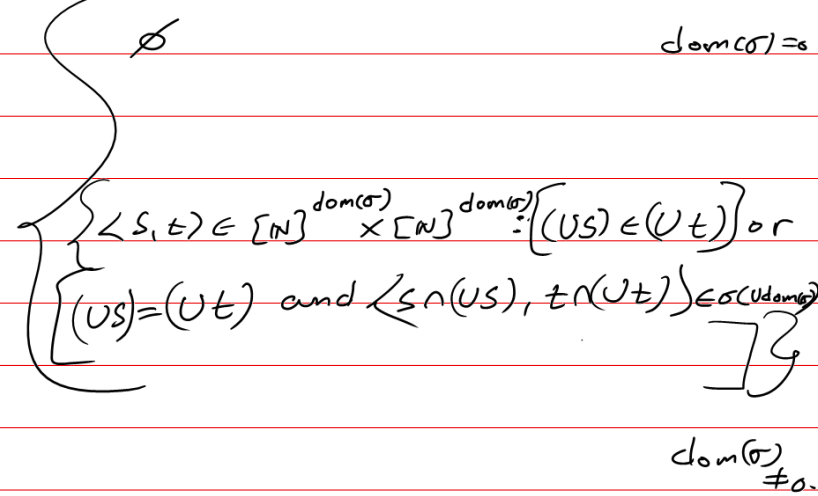
\includegraphics[width=0.49\linewidth]{extender1.png}    
        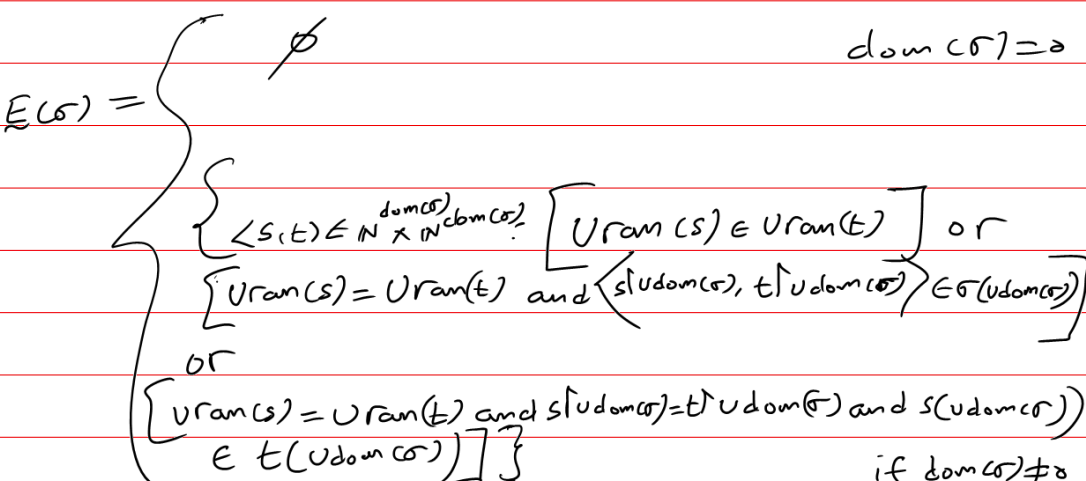
\includegraphics[width=0.49\linewidth]{extender2.png}    
    \end{center}
\end{enumerate}


\subsection{7.2 Sets of Size Continuum}
\textbf{F7.12} If $x, y \in \mathbb{R}$ and $x < y$, there is a $q \in \mathbb{Q}$ with $x < q < y$.

\textbf{L7.13} $2^\mathbb{N} \lessapprox \mathbb{R} \lessapprox \mathcal{P}(\mathbb{Q})$

\textbf{T7.14} These sets are equinumerous: $2^\mathbb{N}$, $\mathbb{N}^\mathbb{N}$, $\mathcal{P}(\mathbb{N} \times \mathbb{N})$, $\mathcal{P}(\mathbb{N})$, $\mathcal{P}(\mathbb{Q})$, $\mathbb{R}$. $2^\mathbb{N} \subseteq \mathbb{N}^\mathbb{N} \subseteq \mathcal{P}(\mathbb{N} \times \mathbb{N})$. So $2^\mathbb{N} \lessapprox \mathbb{N}^\mathbb{N} \lessapprox \mathcal{P}(\mathbb{N} \times \mathbb{N})$. $\mathbb{N} \approx \mathbb{N} \times \mathbb{N}$. By L5.22, $\mathcal{P}(\mathbb{N})\lessapprox \mathcal{P}(\mathbb{N} \times \mathbb{N}) \lessapprox \mathcal{P}(\mathbb{N})$ so $\mathcal{P}(\mathbb{N}) \approx \mathcal{P}(\mathbb{N} \times \mathbb{N})$. By L7.8, $\mathbb{Q} \lessapprox \mathbb{N}$. By F5.2, $2^\mathbb{N} \lessapprox \mathbb{R} \lessapprox \mathcal{P}(\mathbb{Q}) \lessapprox \mathcal{P}(\mathbb{N}) \lessapprox 2^\mathbb{N}$. We also have $2^\mathbb{N} \lessapprox \mathbb{N}^\mathbb{N} \lessapprox \mathcal{P}(\mathbb{N} \times \mathbb{N}) \lessapprox 2^\mathbb{N}$.

\textbf{D7.15} A set $X$ has size continuum or size $\mathfrak{c}$ if $X \approx \mathcal{P}(\mathbb{N})$.

\textbf{L7.16} $(r, s)=\{x \in \mathbb{R} : r < x < s\}$ has size $\mathfrak{c}$. The function $f(x) =
    \left\{
    \begin{array}{lr}
      \frac{x-t}{s-x} & \text{if $x \geq t$} \\
      \frac{x-t}{x-r} & \text{if $x < t$} \\
    \end{array}
    \right.
    $ is well-defined and $1-1$ and onto.

\textbf{E7.17} Let $l \subseteq \mathbb{R}^2$ be a line. Define $\phi:\mathbb{R}\rightarrow l$ as $\phi(x)=\langle x, mx+c\rangle$ and $\phi(y)=\langle c,y \rangle$ for the different line cases. $l \approx \mathbb{R}$. For $a < b$ and $c < d$, let $m=\frac{d-c}{b-a}$ and $p=c-ma$. Then $f:(a, b) \rightarrow (c, d)$ is $1-1$ and onto.

\textbf{E7.19} Prove $\mathbb{N} \times \mathbb{N} \approx \mathbb{N}$. Define $H: \mathbb{N} \times \mathbb{N} \rightarrow \mathbb{N}$ by $H(m, n)=\frac{(m+n)(m+n+1)}{2}+m$. $H$ is $1-1$ and onto by the following steps.
\begin{enumerate}
    \item If $i+j=n$, then $H(i, j)=H(0, n)+i<H(0, n+1)$
    \item If $i+j=n$, $x+y=n$, $i< x$, then $H(i, j) < H(x, y)$
    \item If $i+j=n$, $x+y=m$, $n<m$, then $H(i, j)<H(x, y)$
    \item $H$ is $1-1$
    \item Let $i \in \mathbb{N}$, and $n=min\{k \in \mathbb{N} : 2i < k(k+1)\}$. If $x=i-\frac{n(n-1)}{2}$ and $y=n-1-x$, then $\langle x, y \rangle \in \mathbb{N} \times \mathbb{N}$ and $H(x, y)=i$, and $H$ is onto
\end{enumerate}

\textbf{L7.21} If $A \lessapprox B$ and $A \neq \emptyset$, then there exists an onto $g:B\rightarrow A$.

\textbf{L7.22 (AC)} Suppose $A$ and $B$ are sets and $f: B \rightarrow A$ is onto. Then $A \lessapprox B$.

\textbf{L7.23} Let $A$, $B$, $C$ be sets and suppose $f:C\rightarrow B$ is onto. Then $A^B \lessapprox A^C$.

\textbf{C7.24} If $B \approx C$, then $A^B \approx A^C$.

\textbf{C7.25} If $A \lessapprox D$, $B \lessapprox C$, and $B \neq \emptyset$, then $A^B \lessapprox D^C$.

\textbf{L7.26} There exists a sequence $\langle A_n: n \in \mathbb{N} \rangle$ of pairwise disjoint infinite subsets of $\mathbb{N}$ such that $\bigcup_{n\in \mathbb{N}}A_n=\mathbb{N}$. Define $B_n=\{\langle n, m \rangle:m \in \mathbb{N}\}$, and let $A_n=f^{-1}(B_n)$.

\textbf{L7.27} Suppose $A$, $B$, and $C$ are sets with $B \cap C = \emptyset$. Then $A^B \times A^C \approx A^{B \cup C}$. Define $F:A^B\times A^C \rightarrow A^{B \cup C}$, $F(f, g) = f \cup g$, and show bijectivity.

\textbf{C7.28} $\mathbb{N}^\mathbb{N} \times \mathbb{N}^\mathbb{N} \approx \mathbb{N}^\mathbb{N}$. Define $A \cup B = \mathbb{N}, A \cap B = \emptyset$. Then $\mathbb{N}^A\approx \mathbb{N}^\mathbb{N} \approx \mathbb{N}^B$ and $\mathbb{N}^\mathbb{N}\times\mathbb{N}^\mathbb{N}\approx \mathbb{N}^A\times\mathbb{N}^B\approx \mathbb{N}^{A \cup B}\approx \mathbb{N}^\mathbb{N}$.

\textbf{C7.29} $\mathbb{R}^2$ has size $\mathfrak{c}$. This can be used to count lines and planes. Use $\mathbb{R}^2\approx\mathbb{R}^{\{0\}}\times \mathbb{R}^{\{1\}}\approx \mathbb{R} \times \mathbb{R} \approx \mathbb{N}^\mathbb{N} \times \mathbb{N}^\mathbb{N} \approx \mathbb{N}^\mathbb{N}\approx\mathbb{R}$.

\textbf{EP7.30} Let $\mathfrak{L}$ denote the set of lines in $\mathbb{R}^2$. $\mathfrak{L}=\mathfrak{L}_0\cup \mathfrak{L}_1$ where $\mathfrak{L}_0=\{l : l \text{ satisfies } y = mx+c, m, c, \in \mathbb{R} \}$ and $\mathfrak{L}_1=\{l : l \text{ satisfies } x=c, c, \in \mathbb{R} \}$. Then $\mathfrak{L}_0\approx\mathbb{R}^2\approx \mathbb{R}$ and $\mathfrak{L}_1\approx \mathbb{R}$, so $\mathfrak{L}$ has size $\mathfrak{c}$.

\textbf{L7.31} Let $A$, $B$, $C$ be sets. $A^{(B \times C)}\approx (A^B)^C$. Define $F:A^{(B \times C)} \rightarrow (A^B)^C$ using $F(f):C\rightarrow A^B$ as $F(f)(c)(b)=f(\langle b,c \rangle)$.

\textbf{C7.32} $(\mathbb{N}^\mathbb{N})^\mathbb{N}\approx \mathbb{N}^\mathbb{N}$. Use $(\mathbb{N}^\mathbb{N})^\mathbb{N}\approx \mathbb{N}^{(\mathbb{N} \times \mathbb{N})}$, and $\mathbb{N} \times \mathbb{N} \approx \mathbb{N}$.

\textbf{C7.33} $\mathbb{R}^\mathbb{N}$ has size $\mathfrak{c}$. Use $\mathbb{R}\approx\mathbb{N}^\mathbb{N}$.

\textbf{D7.34} A function $f:\mathbb{R} \rightarrow \mathbb{R}$ is continuous if for each $x \in \mathbb{R}$ and each $\epsilon > 0$, there exists $\delta > 0$ such that $Im_f((x-\delta, x+\delta)) \subseteq (f(x)-\epsilon, f(x)+\epsilon)$. A set $U \subseteq \mathbb{R}$ is an open interval if there exists $r, s \in \mathbb{R}$ such that $U=(r,s)=\{x \in \mathbb{R} : r < x <s\}$. $U \subseteq \mathbb{R}$ is open if it is the union of a collection of open intervals.

\textbf{L7.35} There are only $\mathfrak{c}$ many continuous functions from $\mathbb{R}$ to $\mathbb{R}$.

\textbf{L7.36} There are only $\mathfrak{c}$ many open subsets of $\mathbb{R}$.

\textbf{E7.37} $\mathbb{R}^\mathbb{R}\approx 2^\mathbb{R}$. First, $2^\mathbb{R} \subseteq \mathbb{R}^\mathbb{R}$, so $2^\mathbb{R} \lessapprox \mathbb{R}^\mathbb{R}$. Next, define $f : \mathbb{R} \rightarrow \mathbb{R}$. $f \in \mathbb{R}^\mathbb{R}$, $f \subseteq \mathbb{R} \times \mathbb{R}$, $f \in \mathcal{P}(\mathbb{R} \times \mathbb{R})$. So $\mathbb{R}^\mathbb{R} \subseteq \mathcal{P}(\mathbb{R} \times \mathbb{R})$, and $\mathbb{R}^\mathbb{R} \lessapprox \mathcal{P}(\mathbb{R} \times \mathbb{R}) \approx 2^{\mathbb{R} \times \mathbb{R}} \approx 2^\mathbb{R}$ as $\mathbb{R} \approx \mathbb{R} \times \mathbb{R}$.

\textbf{E7.38} There are only countably many algebraic real numbers. Almost all real numbers are transcendental. $a \in \mathbb{R}$ is algebraic if there exists a non-zero polynomial $p(X) \in \mathbb{Z}[X]$ such that $p(a)=0$. If $a$ is not algebraic, it is transcendental.

\textbf{E7.39} A function $f : \mathbb{R} \rightarrow \mathbb{R}$ is increasing if $\forall x, y, \in \mathbb{R} \ [x \leq y \Rightarrow f(x) \leq f(y)]$. There are only $\mathfrak{c}$ many increasing functions.

\textbf{E7.40} Let $X \subseteq 2^\mathbb{N}$ be countable. Then $(2^\mathbb{N} \backslash X) \approx 2^\mathbb{N}$. If $T$ is the set of transcendental real numbers, $T \approx R$. Since $(2^\mathbb{N} \backslash X) \subseteq 2^\mathbb{N}$, $(2^\mathbb{N} \backslash X) \lessapprox 2^\mathbb{N}$. We want to show that $2^\mathbb{N} \lessapprox (2^\mathbb{N} \backslash X)$ so that we can apply Schröder Bernstein. Let $A, B \subseteq \mathbb{N}$ be infinite sets such that $A \cap B = \emptyset$ and $A \cup B = \mathbb{N}$. By C5.33, fix bijections $\psi : A \rightarrow \mathbb{N}$ and $\varphi : B \rightarrow \mathbb{N}$. Define $G:2^\mathbb{N} \rightarrow (2^\mathbb{N} \backslash X)$ as follows by defining $G(f): \mathbb{N} \rightarrow 2$. Let $n \in \mathbb{N}$. If $n \in A$, define $G(f)(n)=f(\psi(n))\in 2$. If $n \in B$, $e(\varphi(n))\in X \subseteq 2^\mathbb{N}$, and $e(\varphi(n))(n)\in 2$. If $e(\varphi(n))(n)=0$, then $G(f)(n)=1$, if $e(\varphi(n))(n)=1$, then $G(f)(n)=0$. Since either $n \in A$ or $n \in B$, $G(f)(n)\in2$ and $G(f) \in 2^\mathbb{N}$. If $G(f) \in X$, then there exists $k \in \mathbb{N}$ with $e(k)=G(f)$ and $n \in B$ with $\varphi(n)=k$. But since $n \in B$, $G(f)(n) \neq e(\varphi(n))(n)=e(k)(n)=G(f)(n)$, a contradiction. This shows $G(f) \notin X$. Now we show that $G$ is $1-1$. Fix $f \neq f' \in 2^\mathbb{N}$. There exists $k \in \mathbb{N}$ with $f(k) \neq f'(k)$. There exists $n \in A$ with $\psi(n)=k$. $G(f)(n)=f(\psi(n))=f(k)\neq f'(k) =f'(\psi(n))=G(f')(n)$. Then $G(f)\neq G(f')$. We have shown that $2^\mathbb{N} \lessapprox (2^\mathbb{N}\backslash X)$ as needed.

\section{8. More about Partial and Linear Orders}
\subsection{8.1 Dilworth's Decomposition for Finite Partial Orders}
\textbf{T8.1 (Dilworth)} Suppose $\langle X, < \rangle$ is a finite partial order. Let $k(X)=max\{m \in \mathbb{N}:\exists A \subseteq X\ [A \text{ is an antichain in } X\land A \approx m]\}$. $X$ is a union of $k(X)$ disjoint chains.

\textbf{CL8.2} For all $j, j' < n$, if $j \neq j'$, then $x_j$ and $x_{j'}$ are incomparable.

\textbf{CL8.3} $\langle Z, < \rangle$ does not have any $n$-element antichains.

\textbf{E8.4} Suppose $k \in \mathbb{N}$ and $\langle X, < \rangle$ is a finite partial order such that all chains have at most $k$ elements. $X$ is a union of $k$ many antichains.

\textbf{E8.5} Suppose $\langle X, < \rangle$ is a partial order. Suppose $k, l \in \mathbb{N}$. Suppose $\langle X, < \rangle$ has the property that all chains have at most $l$ elements and all antichains have at most $k$ elements. $X$ is finite or it has at most $k \cdot l$ elements.

\textbf{E8.6} Suppose $X$ is a finite set of women and $Y$ is a set of men with $Y \approx n$ for some $n \in \mathbb{N}$. Let the sequence $\langle a_i : i < n \rangle$ enumerate the men. For each $i< n$, $a_i$ chooses a set $S_i \subseteq X$ of women he likes. It is possible to marry each $a_i$ to someone in $S_i$ iff for all $k \leq n$ and all $k$-element subsets $F \subseteq n$, $\bigcup_{i \in F}S_i$ has at least $k$ elements.

\subsection{8.2 More about Linear Orders}
\textbf{D8.8} Let $\langle X, < \rangle$ be a partial order and $A \subseteq X$. $x \in X$ is an upper bound of $A$ if $\forall a \in A \ [a \leq x]$. $x$ is a lower bound if $\forall a \in A \ [x \leq a]$. Let $U$ be the set of upper bounds of $A$ and $L$ be the set of lower bounds of $A$. If there exists $u \in U$ such that $\forall x \in U \ [u \leq x]$, then $u$ is the supremum of $A$ in $X$ or $sup_X(A)$ or minimal upper bound. For $L$ and $[x \leq l]$, it is called the infimum or $inf_X(A)$ or greatest lower bound. There can only be at most one supremum or infimum.

\textbf{EP8.9} Let $A=\{p \in \mathbb{Q} : p^2 < 2\}$. $sup_\mathbb{Q}(A)$ and $inf_\mathbb{Q}(A)$ do not exist, but $sup_\mathbb{R}(A)=\sqrt2$ and $inf_\mathbb{R}(A)=-\sqrt2$.

\textbf{D8.10} Let $\langle X, < \rangle$ be a linear order. A pair $\langle A, B \rangle$ is a cut of $\langle X, < \rangle$ if $A$ is downwards closed, $B$ is upwards closed, and $A$ and $B$ partition $X$ i.e. $A \cap B = \emptyset$ and $A \cup B = X$.

\textbf{F8.11} Suppose $\langle X, < \rangle$ is a linear order and $Y \subseteq X$. If $z \in X \backslash Y$, $A=\{a \in Y:a<z\}$, $B=\{b \in Y: z <b\}$, then $\langle A, B \rangle$ is a cut of $\langle Y, < \rangle$.

\textbf{D8.13} A linear order $\langle X, < \rangle$ is dense if $\forall x, y \in X \ \exists z \in X \ [x < y \Rightarrow x < z < y]$.

\textbf{D8.14} A linear order is without endpoints if it has neither a maximal nor minimal element. A countable dense linear order with no endpoints is universal for all countable linear orders; every countable linear order embeds into such an order.

\textbf{T8.15 (Cantor, AC)} Suppose $\langle X, < \rangle$ is a non-empty dense linear order without endpoints. Let $\langle Y, \prec \rangle$ be any countable linear order. Then $\langle Y, \prec \rangle \hookrightarrow \langle X, < \rangle$.

\textbf{T8.16 (Cantor)} Let $\langle X, < \rangle$ and $\langle Y, \prec \rangle$ be non-empty countable dense linear orders without endpoints. Then they are isomorphic.

\textbf{E8.17} Embedding is a quasi-order (reflexive, transitive) on linear orders.

\textbf{E8.19} $\langle X, < \rangle \hookrightarrow \langle Y, \prec \rangle \land \langle Y, \prec \rangle \hookrightarrow \langle X, < \rangle$ does not imply isomorphism. Take $X=\mathbb{Q} \cap [0, 1]$ and $Y=\mathbb{Q} \cap (0, 1)$.

\textbf{E8.20} We can have $\langle X, < \rangle \not \hookrightarrow \langle Y, \prec \rangle \land \langle Y, \prec \rangle \not \hookrightarrow \langle X, < \rangle$ (incomparability). Take $X=\langle \mathbb{N}, \in \rangle$ and $Y=\langle \mathbb{N}, \ni \rangle$.

\section{9. Well-Ordered Sets}
\textbf{F9.1} If $\langle X, < \rangle$ is a linear order of type $\omega$, then it is a well-order.

\textbf{L9.2} Suppose $A$ and $B$ are downwards closed subsert of $X$ where $\langle X, < \rangle$ is a well-order. If $\langle A, <\rangle\cong\langle B, <\rangle$, then $A=B$.

\textbf{C9.3} Suppose $\langle X, < \rangle$ is a well-order, and $x<x'\in X$. Then $\langle pred_{\langle X, < \rangle}(x'), <\rangle \not\cong \langle pred_{\langle X, < \rangle}(x), <\rangle$.

\textbf{C9.4} Suppose $\langle X, <\rangle$ is a well-order. Then for any $x \in X$, $\langle pred_{\langle X, < \rangle}(x), <\rangle \not \cong \langle X, < \rangle$.

\textbf{L9.5} If $\langle X, < \rangle$ and $\langle Y, \prec \rangle$ are isomorphic well-orders, then the isomorphism between them is unique.

\textbf{T9.6} Suppose $\langle X, < \rangle$ and $\langle Y, \prec \rangle$ are well-orders. Then exactly one of the following holds:
\begin{enumerate}
    \item $\langle X, < \rangle \cong \langle Y, \prec \rangle$
    \item $\exists x \in X\ [\langle pred_{\langle X, <\rangle}(x),< \rangle \cong \langle Y, \prec \rangle]$
    \item $\exists y \in Y\ [\langle X, < \rangle \cong \langle pred_{\langle Y, \prec\rangle}(y),\prec \rangle]$
\end{enumerate}

\textbf{E9.11} Define the product of $X$ and $Y$ to be $Z=Y \times X$. The dictionary order $\lhd$ on $Z$ is a well-order.

\textbf{E9.13} Given well-orders $\langle X, <_X \rangle \cong \langle A, <_A \rangle, \langle Y, <_Y \rangle \cong \langle B, <_B \rangle$, then the product and sum of $\langle X, <_X \rangle, \langle Y, <_Y \rangle \cong \langle A, <_A \rangle, \langle B, <_B \rangle$.

\section{10. Ordinals}
$\mathbf{WO}=\{\langle X, <\rangle : X \text{ is a set }\land<\text{is a well-ordering of }X\}$
\subsection{10.1 Basic Properties of Ordinals}
\textbf{D10.1} A set $x$ is transitive if every element of $x$ is a subset of $x$, or $\forall y \ [y \in x \Rightarrow y \subseteq x]$.

\textbf{D10.2 Ordinals} A set $\alpha$ is an ordinal if it is transitive and well-ordered by $\in$. Let $\in_{\alpha}=\{\langle \beta, \gamma \rangle \in \alpha \times \alpha : \beta \in \gamma\}$. $\alpha$ is an ordinal if $\alpha$ is transitive and $\langle \alpha, \in_{\alpha}\rangle$ is a well-order. The subscript of $\in_\alpha$ is often omitted.

\textbf{F10.3} $\mathbb{N}$ is an ordinal. Every $n \in \mathbb{N}$ is also an ordinal.

\textbf{T10.4} Let $x$ be an ordinal. The following hold:
\begin{enumerate}
    \item $\forall y \in x\ [y \text{ is an ordinal} \land y=pred_{\langle x, \in \rangle}(y)]$
    \item if $y$ is any ordinal and $\langle x,\in\rangle \cong \langle y, \in \rangle$ then $x=y$
    \item if $y$ is any ordinal, then exactly one of the following things hold: $x \in y, x=y, y \in x$
    \item if $y, z$ are ordinals and $x\in y$ and $y \in z$, then $x \in z$
    \item if $\mathbf{C}$ is a non-empty class of ordinals, then $\exists y \in \mathbf{C}\ \forall z \in \mathbf{C}\ [y \in z \lor y =z]$
\end{enumerate}

\textbf{D10.5} $\mathbf{ORD}=\{\alpha:\alpha \text{ is an ordinal}\}$ is the class of all ordinals.

\textbf{T10.6 Burali-Forti} $\mathbf{ORD}$ is not a set.

\textbf{L10.7} Every transitive set of ordinals is an ordinal.

\textbf{T10.8} Let $\langle X, < \rangle$ be a well-ordered set. Then there exists a unique $\alpha$ such that $\langle X,<\rangle\cong\langle\alpha, \in_\alpha\rangle$.

\textbf{D10.11} If $\langle X, <\rangle$ is any well-ordered set, then $otp(\langle X, < \rangle)$, or the order type of $\langle X, < \rangle$ is the unique ordinal $\alpha$ such that $\langle X, <\rangle$ is isomorphic to $\langle \alpha, \in_\alpha\rangle$.

\textbf{L10.13} For ordinals $\alpha, \beta$, $\alpha \leq \beta$ iff $\alpha \subseteq \beta$.

\textbf{L10.14} If $A$ is a non-empty set of ordinals, then $min(A)=\bigcap A$. If $A$ is any set of ordinals, then $sup_{\mathbf{ORD}}(A)=\bigcup A$.

\textbf{L10.15} For any $\alpha$, $S(\alpha)$ is an ordinal, $\alpha < S(\alpha)$, and $\forall\beta\ [\beta<S(\alpha)\Longleftrightarrow \beta \leq \alpha]$.

\textbf{D10.16} $\alpha$ is a successor ordinal if $\exists \beta \ [\alpha=S(\beta)]$. $\alpha$ is a limit ordinal if $\alpha\neq0$ and $\alpha$ is not a successor ordinal.

\textbf{L10.17} An ordinal $\alpha$ is a natural number iff $\forall \beta \leq \alpha \ [\beta=0\lor \beta \text{ is a successor ordinal}]$.

\textbf{CV10.18} $\omega=\mathbb{N}$.

\subsection{Induction and Recursion on the Ordinals}
\textbf{T10.19} Let $P(\alpha)$ be some property. If $\forall \alpha \in \mathbf{ORD}\ [\forall \beta < \alpha\ [P(\beta)] \Longrightarrow P(\alpha)]$ then $\forall \alpha \in \mathbf{ORD}\ [P(\alpha)]$.

\textbf{D10.20} Let $\mathbf{FOD}=\{\sigma:\sigma \text{ is a function }\land \exists \alpha \in \mathbf{ORD} \ [dom(\sigma)=a]\}$ denote the class of all functions whose domain is some ordinal. An ordinal extender is a function $\mathbf{E:FOD\rightarrow V}$. When you plug in a function with domain $\alpha$ into an ordinal extender, the output tells you what the value of the function at $\alpha$ ought to be.

\textbf{T10.21} Suppose $\mathbf{E:FOD\rightarrow V}$ is any extender. Then there exists a unique function $\mathbf{F:ORD\rightarrow V}$ satisfying the condition that $\forall \alpha \in \mathbf{ORD}\ [\mathbf{F}(\alpha)=\mathbf{E(F}\restriction\alpha)]$. The function generated is a proper class and not a set. $\mathbf{F}\restriction\alpha$ is a function with $dom(\mathbf{F}\restriction\alpha)=\alpha$ because $\alpha \subseteq \mathbf{ORD}$.

\textbf{EP10.24} Define $V_0=\emptyset$. Fix $\alpha \in \mathbf{ORD}$ and suppose $V_\beta$ is given for all $\beta<\alpha$. If $\alpha=S(\beta)$ for some $\beta$ let $V_\alpha=\mathcal{P}(V_\beta)$. If $\alpha$ is a limit ordinal, then $V_\alpha=\bigcup\{V_\beta:\beta<\alpha\}$. Define $\mathbf{E:FOD\rightarrow V}$ as follows. Fix $\sigma\in \mathbf{FOD}$. Let $\alpha=dom(\sigma)\in \mathbf{ORD}$. If $\alpha=0, \mathbf{E}(\sigma)=\emptyset$. If $\alpha$ is a successor ordinal, $\exists! \beta, S(\beta)=\alpha$. Then $\beta\in\alpha$, so $\sigma(\beta)$ is defined and in $\mathbf{V}$. Let $\mathbf{E}(\sigma)=\mathcal{P}(\sigma(\beta))$. If $\alpha$ is a limit ordinal, then let $\mathbf{E}(\sigma)=\bigcup ran(\sigma)$.

\textbf{E10.26} Call $\mathbf{C}$ trans-finitely inductive if:
\begin{enumerate}
    \item $0\in \mathbf{C}$
    \item $\forall x \in \mathbf{C} \ [S(x) \in \mathbf{C}]$
    \item for any set $X \subseteq \mathbf{C}, \bigcup X \in \mathbf{C}$
\end{enumerate} $\mathbf{ORD}$ is the smallest trans-finitely inductive class.

\textbf{E10.27} Let $\alpha$ be any ordinal. If $X\subseteq \alpha$, then $otp(\langle X, \in \rangle) \leq \alpha$.

\textbf{E10.28} Let $\alpha$ be any ordinal. $\alpha$ is a limit ordinal iff $\bigcup \alpha=\alpha$.

\textbf{E10.29} For EP10.24, for each $\alpha\in\mathbf{ORD}$, $V_\alpha$ is transitive and $\bigcup_{\alpha\in\mathbf{ORD}}V_\alpha$ is transitive, $\alpha \subseteq V_\alpha$ and $\alpha \notin V_\alpha$.

\section{11. Ordinal Arithmetic}
\subsection{11.1 Addition and Multiplication}
\textbf{D11.1} Let $\langle X, <_X \rangle$ and $\langle Y, <_Y \rangle$ be well-orders. Define $X \oplus Y=(\{0\}\times X)\cup(\{1\}\times Y)$. Define $<_{X\oplus Y}$ to be:
\begin{enumerate}
    \item $\forall x, x' \in X \ [\langle 0, x\rangle <_{X\oplus Y}\langle0, x'\rangle \Longleftrightarrow x <_X x']$
    \item $\forall y, y' \in Y \ [\langle 1, y\rangle <_{X\oplus Y}\langle1, y'\rangle \Longleftrightarrow y <_Y y']$
    \item $\forall x \in X\forall\ y \in Y \ [\langle 0, x\rangle <_{X\oplus Y}\langle1, y\rangle]$
\end{enumerate}
Then it is a well-order.

\textbf{D11.2} Suppose $\alpha$ and $\beta$ are ordinals. Define $\alpha+\beta$ to be the order-type of the well-order $\langle\alpha \oplus\beta, <_{\alpha \oplus \beta}\rangle$, where $<_\alpha=\in_\alpha$ and $<_\beta=\in_\beta$.

\textbf{L11.4} Let $\langle X, <_X \rangle, \langle Y, <_Y \rangle, \langle Z, <_Z\rangle$ be well-orders. Suppose $A,B\subseteq Z$. Assume $A\cup B=Z$ and $\forall a \in A \ \forall b \in B\ [a <_Zb]$. Then if $\langle A, <_Z\rangle \cong \langle X, <_X \rangle$ and $\langle B, <_Z \rangle \cong \langle Y, <_Y \rangle$, then $\langle Z, <_Z \rangle \cong \langle X \oplus Y, <_{X\oplus Y}\rangle$.

\textbf{L11.5} For any $\alpha, \beta, \gamma$:
\begin{enumerate}
    \item $\alpha+(\beta+\gamma)=(\alpha+\beta)+\gamma$
    \item $\alpha+0=\alpha$
    \item $\alpha+1=S(\alpha)$
    \item $\alpha+S(\beta)=S(\alpha+\beta)$
    \item if $\beta$ is a limit ordinal, then $\alpha+\beta=sup\{\alpha+\xi:\xi<\beta\}$
\end{enumerate}

\textbf{R11.6} $(2), (3), (5)$ can be used to give an inductive definition of $+$. For a fixed $\alpha$, we can define $\dotplus$ which is equivalent to $+$ on $\mathbf{ORD}$ by:
\begin{enumerate}
    \item $\alpha\dotplus 0 = \alpha$
    \item $\alpha \dotplus S(\beta)=S(\alpha\dotplus\beta)$
    \item if $\beta$ is a limit ordinal, then $\alpha\dotplus\beta=sup\{\alpha\dotplus\xi:\xi<\beta\}$
\end{enumerate}

\textbf{D11.7} Let $\alpha$ and $\beta$ be ordinals. Let $<_{\alpha\cdot\beta}$ be the dictionary order on $\beta\times \alpha$. That is, for $\langle\zeta, \xi\rangle, \langle \zeta', \xi'\rangle\in\beta \times \alpha$, $\langle \zeta, \xi\rangle <_{\alpha\cdot\beta} \langle\zeta', \xi'\rangle$ iff either $\zeta<\zeta'$ or $\zeta=\zeta'$ and $\xi<\xi'$. Then it is a well-order and $\alpha\cdot\beta=otp(\langle \beta \times \alpha, <_{\alpha\cdot\beta}\rangle)$ which is $\beta$ copies of $\alpha$.

\textbf{L11.8} Suppose $\alpha, \beta, \gamma$ are ordinals. Suppose $A\subseteq\gamma$ and $\langle A, \in \rangle\cong\langle\beta,\in\rangle$. Then $\langle A\times \alpha, <_{\alpha\cdot\gamma}\rangle\cong\langle \beta \times\alpha, <_{\alpha\cdot\beta}\rangle$.

\textbf{L11.9} For any $\alpha, \beta, \gamma$:
\begin{enumerate}
    \item $\alpha \cdot (\beta \cdot \gamma)=(\alpha \cdot \beta)\cdot \gamma$
    \item $\alpha \cdot 0=0$
    \item $\alpha \cdot 1=\alpha$
    \item $\alpha \cdot S(\beta)=a\cdot\beta+\alpha$
    \item if $\beta$ is a limit ordinal, $\alpha\cdot\beta=sup\{a\cdot\xi:\xi<\beta\}$
    \item $\alpha \cdot(\beta+\gamma)=\alpha\cdot\beta+\alpha\cdot\gamma$
\end{enumerate}
Also, $\cdot$ is not commutative on $\mathbf{ORD}$ since $2\cdot \omega\neq\omega\cdot2$. $(6)$ fails for multiplication on the right since $(1+1)\cdot\omega=\omega\neq 1\cdot \omega+1\cdot\omega$.

\subsection{Exponentiation}
\textbf{D11.10} For a fixed $\alpha$, define $\alpha^\beta$ by recursion on $\beta$ using the following clauses:
\begin{enumerate}
    \item if $\alpha=0$,then $\alpha^0=0$; if $\alpha>0$, then $\alpha^0=1$
    \item $\alpha^{\beta+1}=\alpha^\beta\cdot\alpha$
    \item if $\beta$ is a limit ordinal, then $\alpha^\beta=sup\{a^\xi:\xi<\beta\}$
\end{enumerate}

\textbf{E11.11} Define the extender $\mathbf{E_\alpha^+:FOD\rightarrow V}$ as follows. For any $\sigma \in \mathbf{FOD}$, $\mathbf{E_\alpha^+}(\sigma) =
    \left\{
    \begin{array}{lr}
      \alpha & \text{if $dom(\sigma)=0$} \\
      S(\sigma(\beta)) & \text{if $dom(\sigma) =S(\beta)$} \\
      \bigcup ran(\sigma) & \text{if $dom(\sigma)$ is a limit ordinal} \\
    \end{array}
    \right.
    $
    
For other operations need to check the case where $\sigma(\beta)\notin\mathbf{ORD}$.

\textbf{E11.12} For any ordinal $\alpha>0$, $\alpha \cdot \omega > \alpha$.

\textbf{E11.13} $\alpha < \beta \Rightarrow \gamma + \alpha < \gamma +\beta \land \alpha + \gamma \leq \beta +\gamma$ but not $<$ on the second clause.

\textbf{E11.14} If $\alpha \geq \omega$ is an ordinal, then $1+\alpha=\alpha$.

\textbf{E11.15} If $\gamma > 0$, then $\alpha < \beta \Rightarrow \gamma \cdot \alpha < \gamma \cdot \beta \land \alpha \cdot \gamma \leq \beta \cdot \gamma$ but not $<$ on the second clause.

\textbf{E11.16} Let $0<\alpha\leq \beta$ be ordinals. There exist unique $\delta, \xi$ such that $\xi < \alpha$ and $\alpha\cdot\delta+\xi=\beta$.

\textbf{E11.17} $\alpha^{(\beta+\gamma)}=\alpha^\beta\cdot\alpha^\gamma$ for ordinals $\alpha>0$.

\textbf{E11.18} Define $\alpha_0=\omega$ and $\forall n \in \omega, a_{n+1}=\omega^{\alpha_n}$. Let $\epsilon_0=sup\{\alpha_n:n\in\omega\}$. Then $\omega^{\epsilon_0}=\epsilon_0$.

\section{Cardinals and Cardinal Arithmetic}
\textbf{D12.1} A set $X$ is said to be well-orderable if there exists a relation $<\subseteq X \times X$ such that $\langle X, < \rangle$ is a well-order.

\textbf{D12.2} Let $X$ be a well-orderable set. Define the cardinality of $X$, $|X|$, to be the minimal element of $\{\alpha\in\mathbf{ORD}:\alpha\approx X\}$. $|\alpha|$ is defined for every $\alpha\in\mathbf{ORD}$, and $|\alpha|\leq\alpha$.

\textbf{D12.3} $\alpha$ is a cardinal if $|\alpha|=\alpha$.

\textbf{F12.4} If $n\in\omega$, then $n$ is a cardinal. $\omega$ is a cardinal.

\textbf{L12.5} If $|\alpha|\leq\beta\leq\alpha$, then $|\beta|=|\alpha|$.

\textbf{L12.6} A se is finite iff $|X|<\omega$. A set is countable iff $|X|\leq\omega$.

\textbf{D12.7} Let $\kappa$ and $\lambda$ be cardinals. These are well-orderable:
\begin{enumerate}
    \item $\kappa\boxplus\lambda=|(\{0\}\times\kappa)\cup(\{1\}\times\lambda)|$
    \item $\kappa\boxtimes\lambda=|\kappa\times\lambda|$
\end{enumerate}

\textbf{L12.8} Every infinite cardinal is a limit ordinal.

\textbf{T12.9} If $\kappa$ is an infinite cardinal, then $\kappa\boxtimes\kappa=\kappa$.

\textbf{C12.10} Let $\kappa$ and $\lambda$ be infinite cardinals. Then $\kappa\boxplus\lambda=\kappa\boxtimes\lambda=max\{\kappa,\lambda\}$.

\textbf{T12.11} For every set $X$ there is a cardinal $\alpha$ such that there is no 1-1 function $f:\alpha\rightarrow X$.

\textbf{D12.16} For each $\alpha\in\mathbf{ORD}$, $\alpha^+$ is the least cardinal strictly greater than $\alpha$.

\textbf{L12.17} Suppose $\mathbf{F:ORD\rightarrow ORD}$ is a function such that $\forall\alpha,\beta\in\mathbf{ORD}\ [\alpha<\beta\Rightarrow\mathbf{F}(\alpha)<\mathbf{F}(\beta)]$. Then $\forall\beta\in\mathbf{ORD}\ [\beta\leq\mathbf{F}(\beta)]$.

\textbf{D12.18} Define a sequence $\langle \omega_\alpha: \alpha \in \mathbf{ORD}\rangle$ by induction using the following clauses:
\begin{enumerate}
    \item $\omega_0=\omega$
    \item $\omega_{S(\alpha)}=\omega_\alpha^+$
    \item if $\alpha$ is a limit ordinal, then $\omega_\alpha=sup\{\omega_\xi:\xi<\alpha\}$
\end{enumerate}

\textbf{R12.19} $\omega_\alpha$ is sometimes deonted as $\aleph_\alpha$.

\textbf{L12.20} $\alpha<\beta\Longrightarrow\aleph_\alpha<\aleph_\beta$ and every infinite cardinal is equal to $\aleph_\alpha$ for some $\alpha\in\mathbf{ORD}$.

\subsection{12.1 Choice and Cardinality}
\textbf{D12.21} Let $X$ be any set. $F$ is a choice function on $X$ if $F$ is a function, $dom(F)=X\backslash\{0\}$, and $\forall a \in X\backslash\{0\}[F(a)\in a]$.

\textbf{T12.22 Zermelo} TFAE for a set $X$:
\begin{enumerate}
    \item $X$ is well-orderable
    \item there exists a choice function on $\mathcal{P}(X)$
\end{enumerate}

\textbf{T12.26 AC} TFAE:
\begin{enumerate}
    \item the Cartesian product of non-empty sets is non-empty
    \item for every set $X$ there exists a choice function on $X$
    \item every set is well-orderable
    \item for any two sets $X$ and $Y$, either $X\lessapprox Y$ or $Y\lessapprox X$
    \item for every set $X$ there is an ordinal $\alpha$ and a 1-1 function $f:X\rightarrow \alpha$
    \item for every set $X$ there is a cardinal $\kappa$ such that $X\approx\kappa$
\end{enumerate}

\subsection{Cardinal Exponentiation and König's Theorem}
\textbf{D12.28 (AC)} Let $\kappa$ and $\lambda$ be cardinals. Define $\kappa^\lambda=|\{f:f\text{ is a function}\land dom(f)=\lambda\land ran(f)\subseteq\kappa\}|$.

\textbf{L12.30} Let $\kappa, \lambda, \theta$ be cardinals. The following hold:
\begin{enumerate}
    \item $(\kappa^\lambda)^\theta=\kappa^{(\lambda\boxtimes\theta)}$
    \item $(\kappa^\lambda)\boxtimes(\kappa^\theta)=\kappa^{(\lambda\boxplus\theta)}$
\end{enumerate}

\textbf{D12.31} Define a squence of cardinals $\langle\beth_\alpha:\alpha\in\mathbf{ORD}\rangle$ by induction using the following clauses:
\begin{enumerate}
    \item $\beth_0=\omega$
    \item $\beth_{S(\alpha)}=2^{\beth_\alpha}$
    \item if $\alpha$ is a limit ordinal, then $\beth_\alpha=sup\{\beth_\xi:\xi<\alpha\}$
\end{enumerate}

\textbf{D12.32} The Generalised Continuum Hypothesis is the statement that $\forall \alpha \in \mathbf{ORD}\ [\beth_\alpha=\aleph_\alpha]$. The Continuum Hypothesis is the statement that $\beth_1=\aleph_1$. Note $\beth_1=2^{\beth_0}=2^{\aleph_0}$, so CH says $2^{\aleph_0}=\aleph_1$.

\textbf{T12.34 König} $(\aleph_\omega)^{\aleph_0}>\aleph_\omega$.

\textbf{C12.35} $2^{\aleph_0}\neq\aleph_\omega$.

\textbf{E12.36} Let $\kappa,\lambda$ be infinite cardinals where $\lambda \leq \kappa$. Then $\kappa^\lambda=|\{X\subseteq\kappa:|X|=\lambda\}|$.

\textbf{E12.37} Let $\kappa, \lambda, \theta, \chi$ be cardinals. If $\kappa \leq \lambda$, then $\kappa^\theta \leq \lambda^\theta$. If $\kappa\leq\chi, \lambda \leq \theta$ and $\lambda\neq0$, then $\kappa^\lambda \leq \chi^\theta$.

\textbf{E12.38} Let $\alpha$ be an ordinal. Let $W = \{\langle Y, \lhd \rangle : Y \subseteq \alpha \land \langle Y, \lhd \rangle \text{ is a well-order}\}$. $\alpha^+=\{otp(\langle Y, \lhd \rangle):\langle Y, \lhd \rangle \in W\}$.

\textbf{E12.39} There is a cardinal $\kappa=\aleph_\kappa$ and $\kappa=\beth_\kappa$.

\textbf{E12.40} Suppose $\mathbf{F:ORD\rightarrow ORD}$ and $\forall \alpha, \beta \in \mathbf{ORD} \ [\alpha < \beta \Longrightarrow \mathbf{F}(\alpha)<\mathbf{F}(\beta)]$ and for any limit ordinal $\beta$, $\mathbf{F}(\beta)=sup\{\mathbf{F}(\alpha):\alpha<\beta\}$. Then $\forall \alpha \in \mathbf{ORD}\ \exists \beta > \alpha \ [\mathbf{F}(\beta)=\beta]$.

\textbf{E12.41} $(\aleph_{\omega_1})^{\aleph_1}>\aleph_{\omega_1}$ and $2^{\aleph_1}\neq\aleph_\omega, \aleph_{\omega_1}$.

\section{13. Some applications of AC}
\textbf{D13.1} Let $A$ be any set. $\mathcal{F}\subseteq\mathcal{P}(A)$ is of finite character iff $\forall X \subseteq A,X\in\mathcal{F}\Longleftrightarrow \forall Y \subseteq X\ [|Y|<\omega\Longrightarrow Y\in\mathcal{F}]$. All of $X$'s finite subsets are in $\mathcal{F}$.

\textbf{L13.2} Suppose $\mathcal{F}\subseteq\mathcal{P}(A)$ is of finite character. Then for any $X\in\mathcal{F}$ and any $Y\subseteq X$, $Y\in\mathcal{F}$.

\textbf{T13.3} TFAE:
\begin{enumerate}
    \item AC
    \item for any set $A$ and any $\mathcal{F}\subseteq\mathcal{P}(A)$, if $F$ has finite character, then for every $X \in \mathcal{F}$, there exists $Y\in\mathcal{F}$ such that $X\subseteq Y$ and $Y$ is maximal in $\langle\mathcal{F},\subsetneq\rangle$ (Teichmüller-Tukey Lemma)
    \item every chain in every partial order is contained in a maximal chain (Hausdorff's maximal chain theorem)
    \item if $\langle X, < \rangle$ is any partial order where every chain in $\langle X, < \rangle$ has an upper bound in $\langle X, <\rangle$, then $\langle X, <\rangle$ has a maximal element (Zorn's lemma)
\end{enumerate}
$(4) \Longrightarrow (1)$: Prove the standard version of AC. Let $I$ be any set and suppose $\langle X_i:i \in I\rangle$ is any sequence of non-empty sets. Consider $A=\{\sigma:\sigma \text{ is a function}\land dom(\sigma)\subseteq I \land \forall i \in dom(\sigma)\ [\sigma(i)\in X_i]\}$. Partially order $A$ by $\subsetneq$. Let $C\subseteq  A$ be any chain. $C$ is a directed collection of functions. So $\bigcup C=\tau$ is a function and $dom(\tau)=\bigcup\{dom(\sigma):\sigma\in C\}\subseteq I$. $\tau(i)=\sigma(i)\in X_i$. Therefore $\tau\in A$ and $\forall \sigma \in C\ [\sigma\subseteq \tau]$. So $\tau$ is an upper bound for $C$. So every chain has an upper bound and there is a maximal $\sigma\in A$ by Zorn's lemma. We claim that $dom(\sigma)=I$. If not, there exists $i\in I \backslash dom(\sigma)$. Since $X_i\neq0$, choose $x_i\in X_i$. Put $\tau=\sigma\cup\{\langle i, x_i\rangle\}$. Then $\tau \in A$ and $\sigma \subsetneq \tau$, contradicting maximality of $\sigma$.

\textbf{Using Zorn's Lemma} $\langle X, < \rangle$ is a partial order. If every chain in $\langle X, < \rangle$ has an upper bound in $\langle X, < \rangle$, then $\langle X, < \rangle$ has a maximal element.
\begin{enumerate}
    \item Find a relevant $\langle X, < \rangle$, e.g. $\langle \mathcal{P}(X), \subsetneq \rangle$ which might be given.
    \item Take a chain $\zeta \subseteq X$. Show $\zeta$ has an upper bound in $\langle X, < \rangle$. Usually this involves taking unions of things in $\zeta$. But you have to check that these unions belong to $X$. Also, $\zeta=\emptyset$ is always a chain.
    \item By Zorn's lemma $\exists x \in X$ maximal in $\langle X, < \rangle$. Now maximality will imply $x$ has some special property. Most of the time you check $x$ has the relevant property, because if it did not it would contradict maximality in $\langle X, < \rangle$.
\end{enumerate}

\textbf{E13.16} Let $\langle X, < \rangle$ be a partial order. Every antichain in $\langle X, < \rangle$ is contained in a maximal antichain. Let $A \subseteq X$ be an antichain.
\begin{enumerate}
    \item $P=\{B\subseteq X:A\subseteq B\land B\text{ is an antichain}\}$. $\langle P, \subsetneq\rangle$ is a partial order.
    \item Let $\zeta \subseteq P$ be a chain in $\langle P, \subsetneq\rangle$. Case I: $\zeta=\emptyset$. Then $A\in P$ and $\forall B \in \zeta \ [B \subseteq A]$. So $A$ is an upper bound for $\zeta \in P$. Case II: $\zeta\neq\emptyset$. Let $D=\bigcup \zeta$. For any $B \in \zeta, B\subseteq D$. If $D \in P$, then $D$ would be an upper bound of $\zeta$ as $\forall B \in \zeta \ [B\subseteq D]$. So We want to show $D \in P$. $D\subseteq X$ as $\forall B \in \zeta \ [B \subseteq X]$. As $\zeta \neq \emptyset$, $\exists B \in \zeta$ such that $A\subseteq B \subseteq D$. So $A \subseteq D$. Show $D$ is an antichain. Suppose $x, y \in D, x\neq y$. $\exists B, B' \in \zeta$ with $x\in B, y \in B'$. As $\zeta$ is a chain, WLOG $B \subseteq B'$. So $x, y \in B'$. Since $B'$ is an antichain, $x \not< y, y \not< x$. So $D$ is an antichain and $D \in P$.
    \item By Zorn's, $\exists B \in P$ which is maximal in $\langle P, \subsetneq \rangle$. Now $A \subseteq B$, $B$ is an antichain. If $\exists D, B \subsetneq D$, then $D \in P$ as $A \subseteq B \subseteq D$, contradicting maximality of $B$ in $\langle P, \subsetneq \rangle$.
\end{enumerate}

\textbf{E13.19} Show every vector space $V$ has a basis. Let $P=\{B\in\mathcal{P}(V):B \text{ is linearly independent}\}$. Then $\langle P, \subsetneq \rangle$ is a partial order. Take $\zeta \subseteq P$. If $\zeta=\emptyset$, then it is an upper bound. If $\zeta\neq\emptyset$, then take $B=\bigcup \zeta$. Suppose $B$ is not linearly independent. Then there is a non-trivial solution, some $X \in \zeta$ must be linearly dependent, violating $X\in \zeta \in P$. So by Zorn's, there exists a maximal element in $B \in P$. Now show $span(B)=V$. Suppose otherwise. Then $\exists v \in V\notin span(B)$. Then take $B \cup \{v\}$ which is linearly independent, but this contradicts maximality of $B$. So $span(B)=V$, and $B$ is a basis of $V$. 

\textbf{23/24 Q5} Call $X \subseteq \mathbb{R}$ an S-$set$ if $\forall w, x, y, z\in X\ [w+x=y+z\Longrightarrow\{w, x\}=\{y,z\}]$. Let $\mathcal{P}=\{X\subseteq \mathbb{R} : X \text{ is an S-$set$}\}$.
\begin{enumerate}
    \item $\langle \mathcal{P}, \subsetneq \rangle$ is a partial order.
    \item Let $\zeta \subseteq \mathcal{P}$ be a chain in $\langle \mathcal{P}, \subsetneq \rangle$. Let $Y=\bigcup \zeta$. $Y \subseteq \mathbb{R}$ as $\forall x \in \zeta[x\subseteq \mathbb{R}]$. Show $Y$ is an S-$set$. Suppose $w, x, y, z \in Y$. Find $w\in X_1, x \in X_2, y \in X_3, z \in X_4$. As $\zeta$ is a chain, WLOG $X_1\subseteq X_2\subseteq X_3 \subseteq X_4$. Then $w,x,y,z\in X_4$. As $X_4 \in \mathcal{P}$, it is an S-$set$. So $Y$ is an S-$set$ and $Y\in\mathcal{P}$. Since $\forall x \in \zeta \ [x \subseteq Y]$, $Y$ is an upper bound for $\zeta$ in $\langle \mathcal{P}, \subsetneq \rangle$.
    \item Show there is an uncountable S-$set$. By Zorn's, let $X \in \mathcal{P}$ be maximal in $\langle \mathcal{P}, \subsetneq \rangle$. Assume $X$ is countable. Let $Y=\{\frac{w+x}{2}:w,x \in X\}, Z=\{w+x-y:w,x,y\in X\}$. $X\cup Y\cup Z$ is countable. As $\mathbb{R}$ is uncountable, let $v\in \mathbb{R} \backslash (X\cup Y \cup Z)$. Then $X\cup\{v\}$ is an S-$set$ by case bashing, and $X\cup\{v\}\in \mathcal{P}$, but this contradicts maximality of $X$.
\end{enumerate}

\textbf{23/24 Q4} $\mathbf{F}(0)=1$, $\mathbf{F}(\beta)=\mathbf{F}(\alpha)\cdot\beta$ if $\beta=\alpha+1$, $\mathbf{F}(\beta)=sup\{\mathbf{F}(\alpha):\alpha<\beta\}$ if $\beta$ is a limit ordinal. The extender is $\mathbf{E}(\sigma) =
    \left\{
    \begin{array}{lr}
      1 & \text{if $dom(\sigma)=0$} \\
      \sigma(\bigcup dom(\sigma))\cdot dom(\sigma) & \text{if $dom(\sigma) =S(\beta)$} \\
      \bigcup ran(\sigma) & \text{if $dom(\sigma)$ is a limit ordinal} \\
      \emptyset & \text{otherwise}\\
    \end{array}
    \right.
    $

Swap out $\beta=dom(\sigma)$, $\mathbf{F}(\alpha)=\sigma(\bigcup dom(\sigma))$ where $\beta=\alpha+1$, $sup...=\bigcup ran(\sigma)$

% \begin{center}
%     \begin{tabular}{lll}
%     \raisebox{-.5\height}{
\includegraphics[scale=0.4]{dilip.jpg}} & pls give me A+ prof thanks \\
%     \end{tabular}
% \end{center}

\end{multicols*}

\end{document}